\documentclass[11pt,a4paper]{report}
\usepackage[utf8]{inputenc}
\usepackage[portuguese]{babel}
\usepackage[T1]{fontenc}
\usepackage{amsmath}
\usepackage{amsfonts}
\usepackage{amssymb}
\usepackage{graphicx}
\title{Relatório sobre o ajuste dos offsets dos satélites irregulares}
\author{Altair Ramos}
\begin{document}
\maketitle

\chapter*{Ajuste}

\indent \indent O problema consiste em ajustar uma função dependente do tempo e da anomalia verdadeira aos offsets obtidos e publicados no artigo de posições dos satélites irregulares. Assim estimando correções às posições dos satélites para predição de ocultações estelares.

As equações utilizadas são as seguintes e dependem da situação:

\begin{equation}
F(t,f) = p[0]\times \frac{t - 2451544.5}{365.65} + p[1]\times \sin(f) + p[2]\times\cos(f) + p[3],
\label{eq:linear}
\end{equation}

\begin{equation}
F(t,f) = p[0]\times\sin\left(\frac{2\pi}{p[1]}\times \frac{t - 2451544.5}{365.25} + p[2]\right) + p[3]\times\sin(f) + p[4]\times\cos(f) + p[5],
\label{eq:sin}
\end{equation}

\begin{equation}
F(t,f) = p[0]\times\cos\left(\frac{2\pi}{p[1]}\times \frac{t - 2451544.5}{365.25} + p[2]\right) + p[3]\times\sin(f) + p[4]\times\cos(f) + p[5],
\label{eq:cos}
\end{equation}
onde $t$ é o tempo em data juliana, $f$ é a anomalia verdadeira e p[i] são os parâmetros de ajuste onde i é o número do parâmetro.

A equação \ref{eq:linear} é basicamente uma variação linear com o tempo mais variações senoidais dependentes da anomalia verdadeira. p[0] foi colocado de forma a ter a unidade de mas/ano. Apenas o ajuste para a declinação de Carme foi utilizada essa função.

As equaç\~oes \ref{eq:sin} e \ref{eq:cos} correspondem a uma variação senoidal com o tempo (uma utilizando o seno e outra o cosseno) mais variações senoidais da anomalia verdadeira. Pra maioria dos casos as duas últimas dão o mesmo resultado. p[1] foi colocado de forma a ser o período da oscilação em anos.

Para cada satélite há quatro gráficos, dois para RA e dois para DEC. Dos pares, um é \textit{offset X tempo} com os ajustes. O outro é \textit{offset X anomalia verdadeira}. Além disso, temos tabelas com os valores e erros obtidos para os parâmetros através do método de mínimos quadrados não-linear.

Nos gráficos em função do tempo, as linhas verticais marcam os instantes de anomalia verdadeira igual a zero (periastro). A linha verde é o ajuste utilizando $1 / \sigma^{2}$ como peso onde $\sigma$ é a dispersão da noite. A linha vermelha é o ajuste dos offsets onde todos os offsets tem o mesmo peso.

Nas tabelas temos os valores derivados para os parâmetros e seus erros a partir dos dois ajustes (com peso e sem peso). Além disso, também mostro o resíduo médio de cada ajuste calculado a partir da seguinte equação:

\begin{equation}
RM = \sqrt{\frac{\sum\limits_{i=1}^{n}{(x_{i} - F(t_{i},f_{i}))^2}w_{i}}{\sum\limits_{i=1}^{n}{w}_{i}}},
\end{equation}
onde $x_{i}$ é o offset, F é a função ajustada para tempo $t_{i}$ e anomalia verdadeira $f_{i}$ e $w_{i}$ é o peso do offset $i$, $n$ é o númrro total de offsets.

Começo apresentando para os satélites de Júpiter. Primeiro os satélites que são únicos de seu grupo orbital e por fim para o grupo de Himalia. Notem que muitos desses ajustes obtêm como período na senoide do tempo um valor entre 10 e 13 anos. Lembrando que o período da órbita de Júpiter é 11.8 anos. Para Phoebe e Nereida, coloquei como chute inicial para o período 1 ano de forma a tentar obter uma variação de paralaxe da Terra, já que não temos observações suficientes para obter uma senoide cujo período seja da ordem da órbita dos planetas Saturno (29.4) e Netuno (164.8).

Ainda precisamos melhorar os ajustes, talvez limitando o peso para que noites com dispersão muito baixa não crie um erro no ajuste ou eliminando offsets com resíduo maior que 2$\sigma$ do resíduo médio. Outra possibilidade é mudar as funções em relação à anomalia verdadeira e/ou ao tempo.


\chapter*{Sinope}

\indent \indent Número total de noites: 36.

\section*{Ascensão Reta}

\indent \indent Para Sinope (RA), o ajuste foi feito utilizando a função \ref{eq:sin}. Vemos pelo gráfico em função do tempo e a tabela que a variação em função da anomalia verdadeira influencia menos que o tempo.\\

\begin{figure}[h]
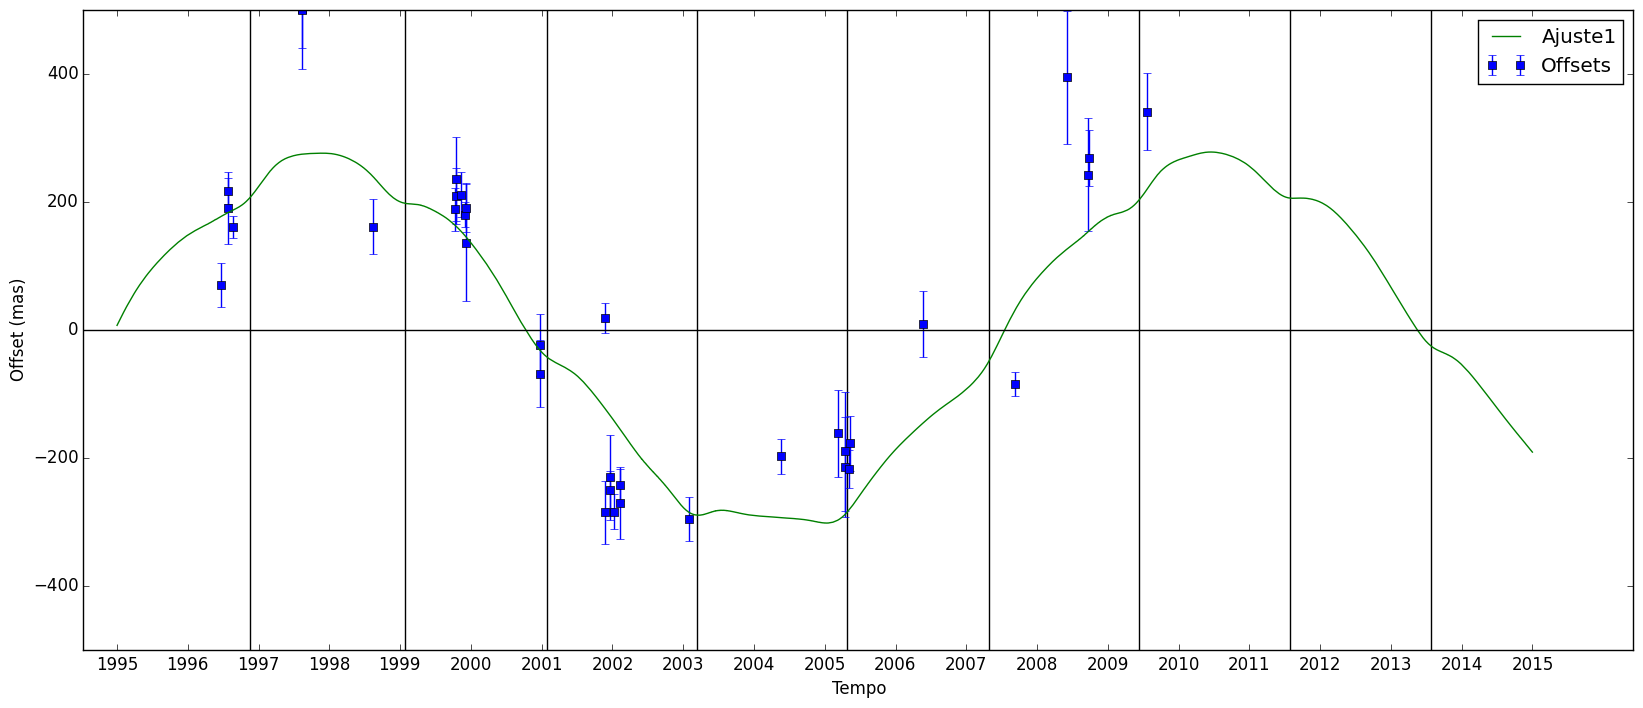
\includegraphics[scale=0.45]{Sinope/RA.png} 
\end{figure}

\begin{figure}[h]
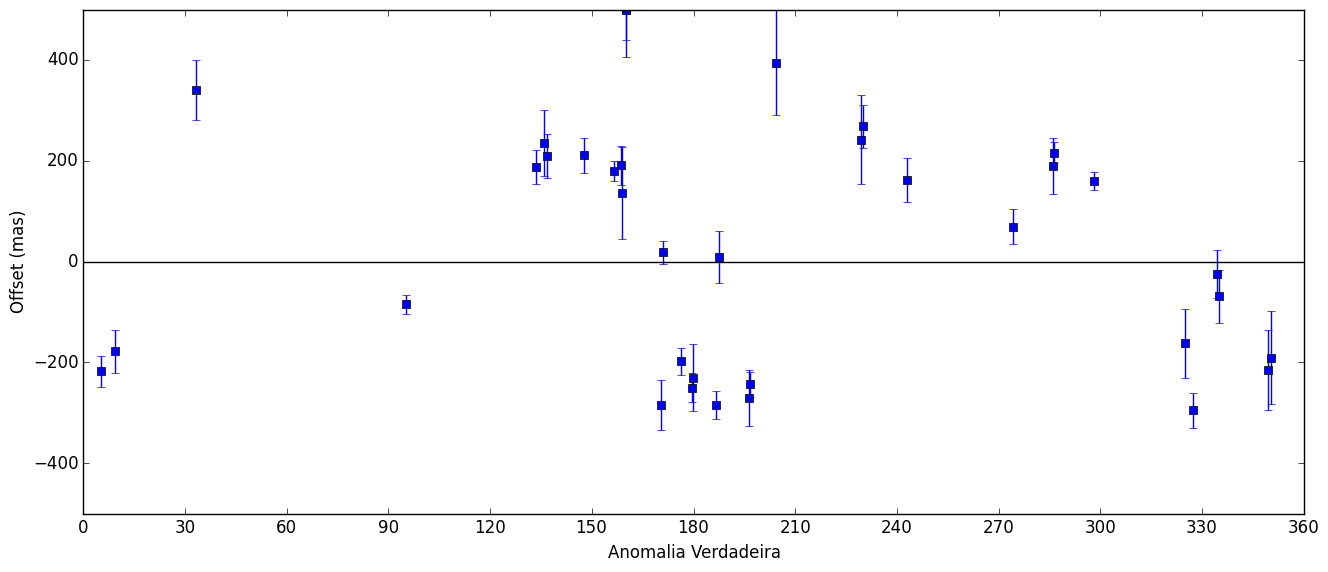
\includegraphics[scale=0.45]{Sinope/RA_anom.png}  
\end{figure}


\begin{table}[h!]
\caption{\label{Tab: Sinope-RA} Resultados dos ajustes para Sinope - RA}
\begin{centering}
\begin{tabular}{cccc}
\hline
\hline
Parâmetro & Com peso & Sem peso & Unidade\tabularnewline
\hline
p[0] & -284 $\pm$ 28 & -316 $\pm$ 25 & mas\\
p[1] & 12 $\pm$ 1 & 11.7 $\pm$ 0.7 & anos\\
p[2] & -30 $\pm$ 8 & -22 $\pm$ 7 & graus\\
p[3] & 10 $\pm$ 48 & 44 $\pm$ 37 & mas\\
p[4] & -15 $\pm$ 31 & -18 $\pm$ 24 & mas\\
p[5] & -26 $\pm$ 21 & 1 $\pm$ 21 & mas\\
Residuo & 91 & 88 & mas\\
\hline 
\end{tabular} 
\par\end{centering}
\end{table}

\section*{Declinação}

\indent \indent Para Declinação também foi utilizada a função \ref{eq:sin}. Nesse, o seno da anomalia verdadeira tem uma importância maior que para RA e que a amplitude do tempo é bem menor que para RA.

\begin{figure}[h]
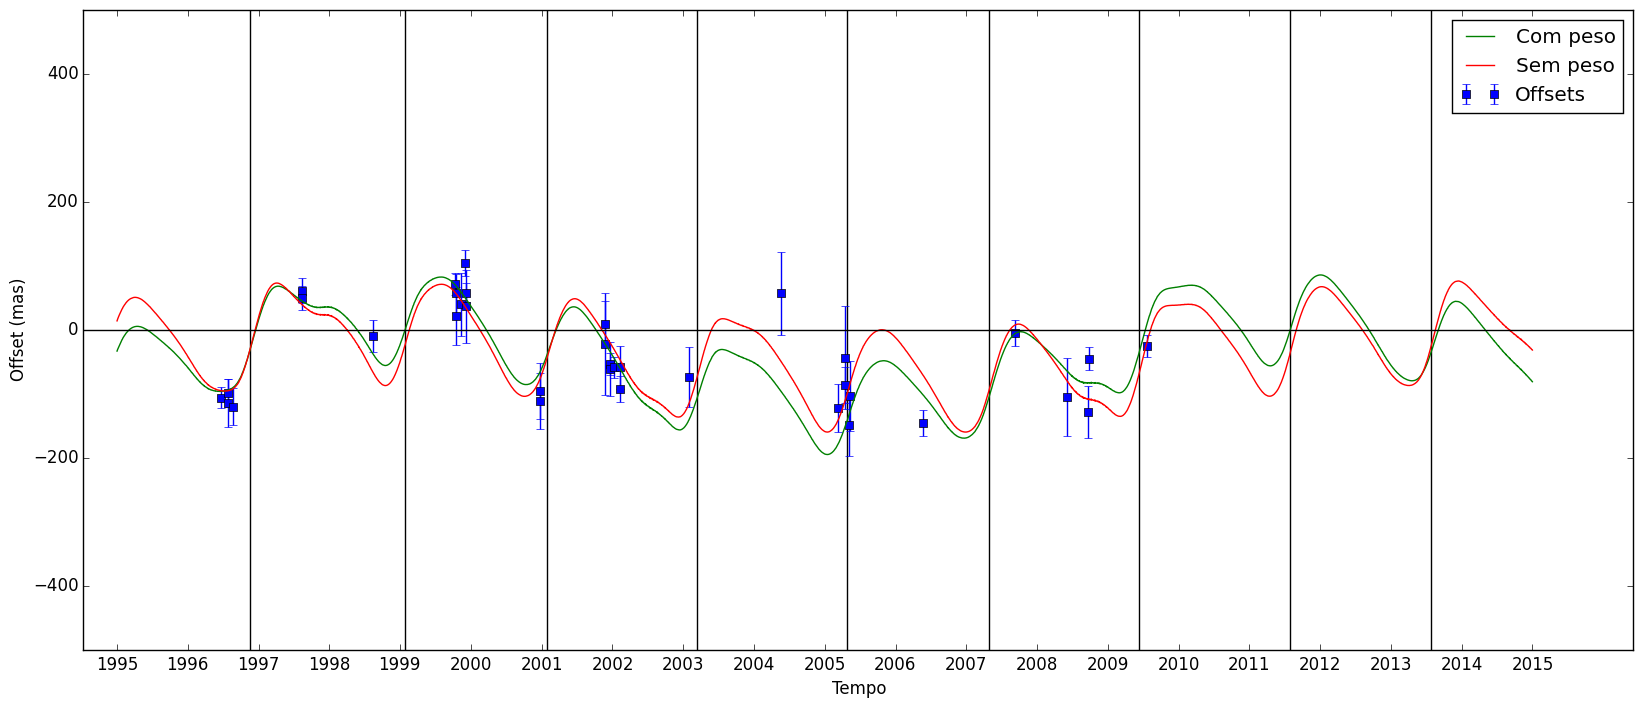
\includegraphics[scale=0.45]{Sinope/DEC.png} 
\end{figure}

\begin{figure}[h]
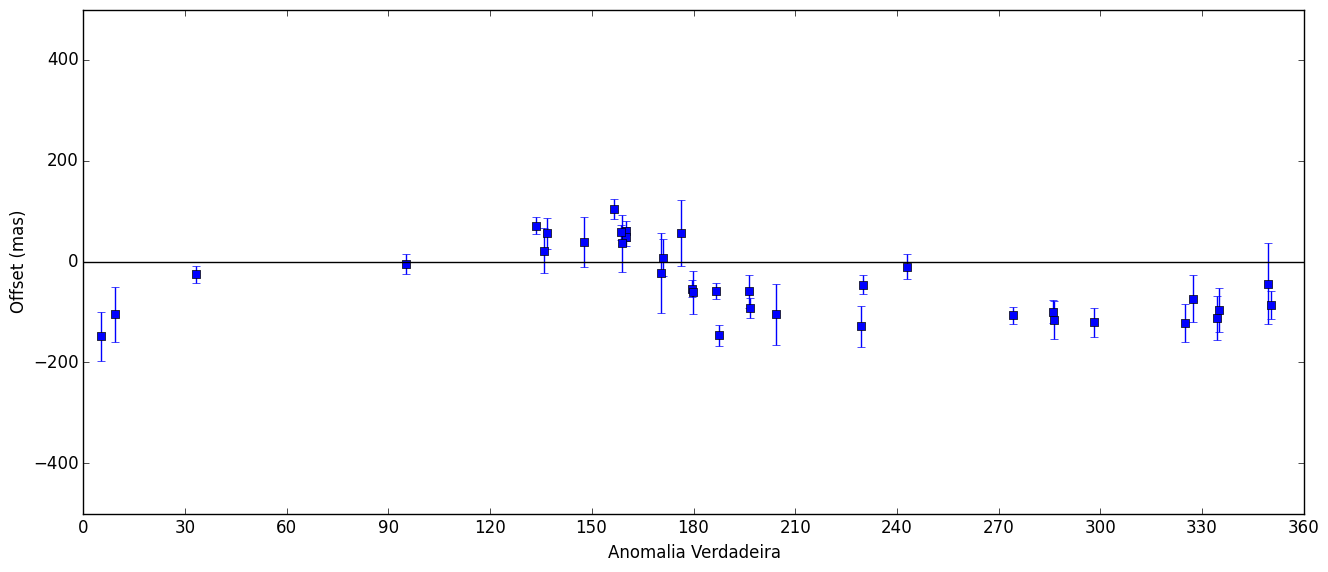
\includegraphics[scale=0.45]{Sinope/DEC_anom.png}  
\end{figure}

\begin{table}[h!]
\caption{\label{Tab: Sinope-DEC} Resultados dos ajustes para Sinope - DEC}
\begin{centering}
\begin{tabular}{cccc}
\hline
\hline
Parâmetro & Com peso & Sem peso & Unidade\tabularnewline
\hline
p[0] & -69 $\pm$ 11 & -38 $\pm$ 11 & mas\\
p[1] & 12.7 $\pm$ 0.7 & 15 $\pm$ 3 & anos\\
p[2] & 123 $\pm$ 8 & 129 $\pm$ 23 & graus\\
p[3] & 69 $\pm$ 11 & 79 $\pm$ 15 & mas\\
p[4] & -18 $\pm$ 9 & -19 $\pm$ 10 & mas\\
p[5] & -54 $\pm$ 7 & -43 $\pm$ 8 & mas\\
Residuo & 30 & 38 & mas\\
\hline 
\end{tabular} 
\par\end{centering}
\end{table}

\chapter*{Pasiphae}

\indent \indent Número total de noites: 65.

\section*{Ascensão Reta}

Foi utilizada a equação \ref{eq:sin}.

\begin{figure}[h]
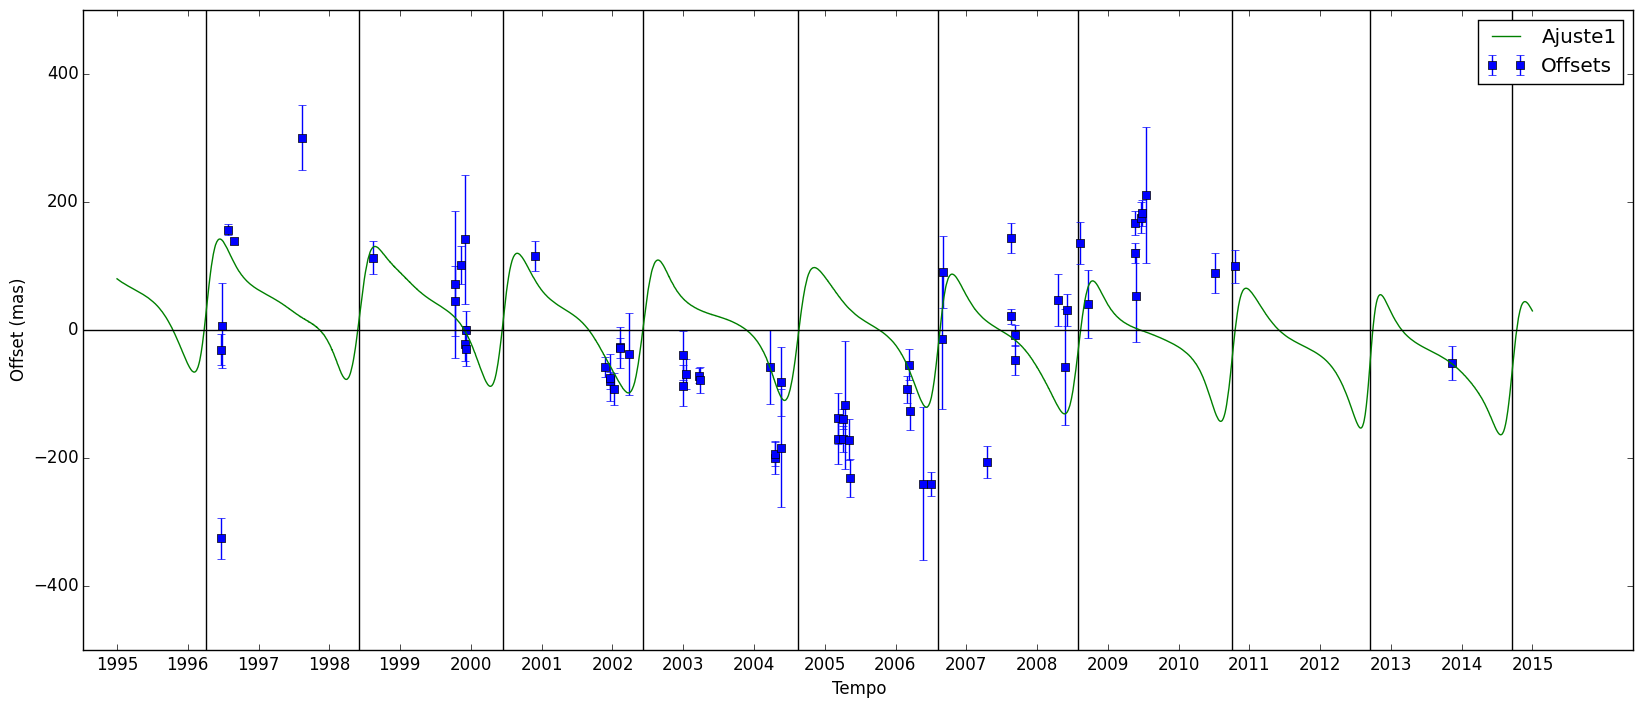
\includegraphics[scale=0.45]{Pasiphae/RA.png} 
\end{figure}

\begin{figure}[h]
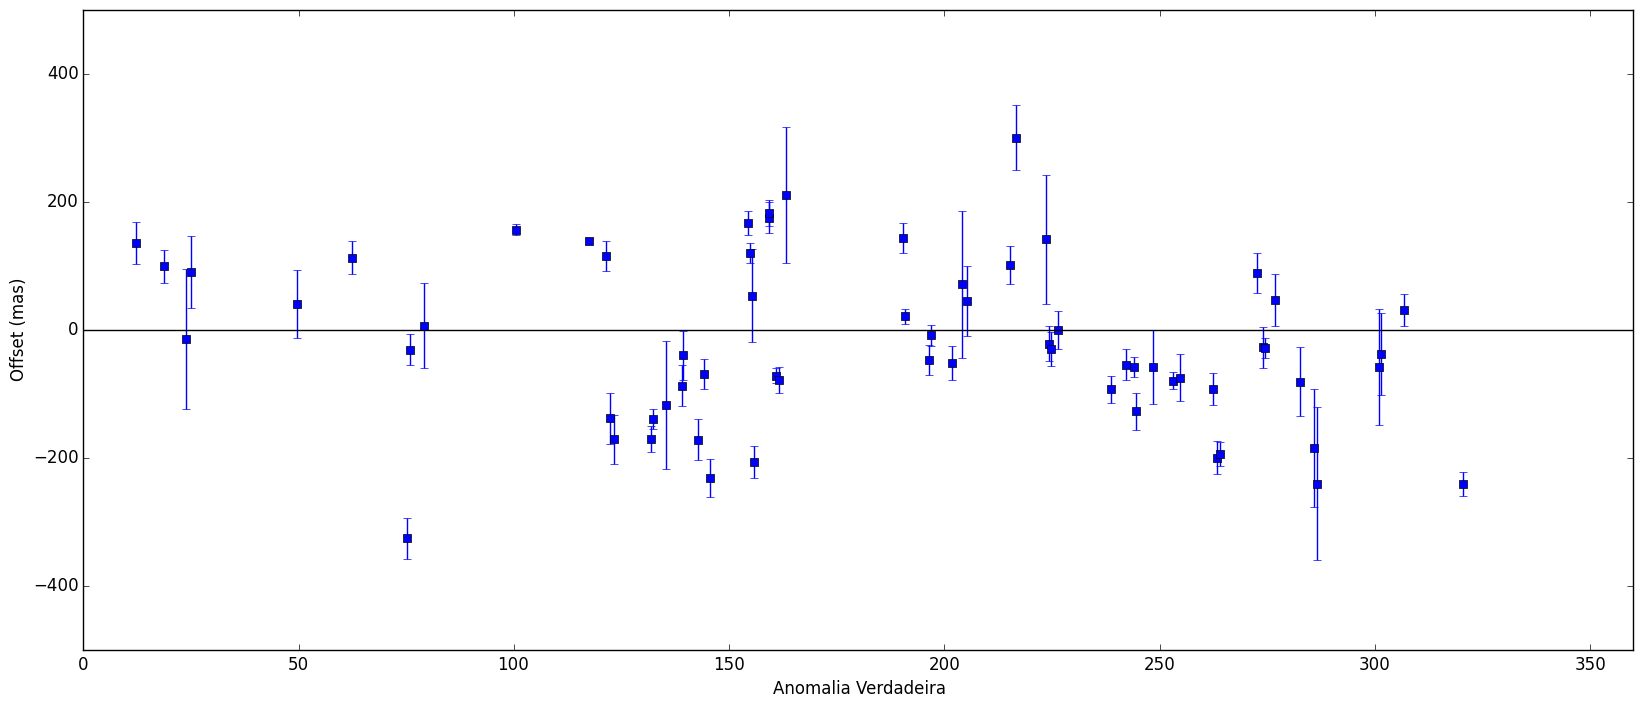
\includegraphics[scale=0.45]{Pasiphae/RA_anom.png}  
\end{figure}

\begin{table}[h!]
\caption{\label{Tab: Pasiphae-RA} Resultados dos ajustes para Pasiphae - RA}
\begin{centering}
\begin{tabular}{cccc}
\hline
\hline
Parâmetro & Com peso & Sem peso & Unidade\tabularnewline
\hline
p[0] & -157 $\pm$ 14 & -136 $\pm$ 15 & mas\\
p[1] & 12.7 $\pm$ 0.4 & 11.3 $\pm$ 0.6 & anos\\
p[2] & -39 $\pm$ 7 & -57 $\pm$ 10 & graus\\
p[3] & 20 $\pm$ 16 & 15 $\pm$ 17 & mas\\
p[4] & -39 $\pm$ 19 & -16 $\pm$ 19 & mas\\
p[5] & -17 $\pm$ 12 & -24 $\pm$ 13 & mas\\
Residuo & 57 & 84 & mas\\
\hline 
\end{tabular} 
\par\end{centering}
\end{table}

\section*{Declinação}

Foi utilizada a equação \ref{eq:sin}.

\begin{figure}[h]
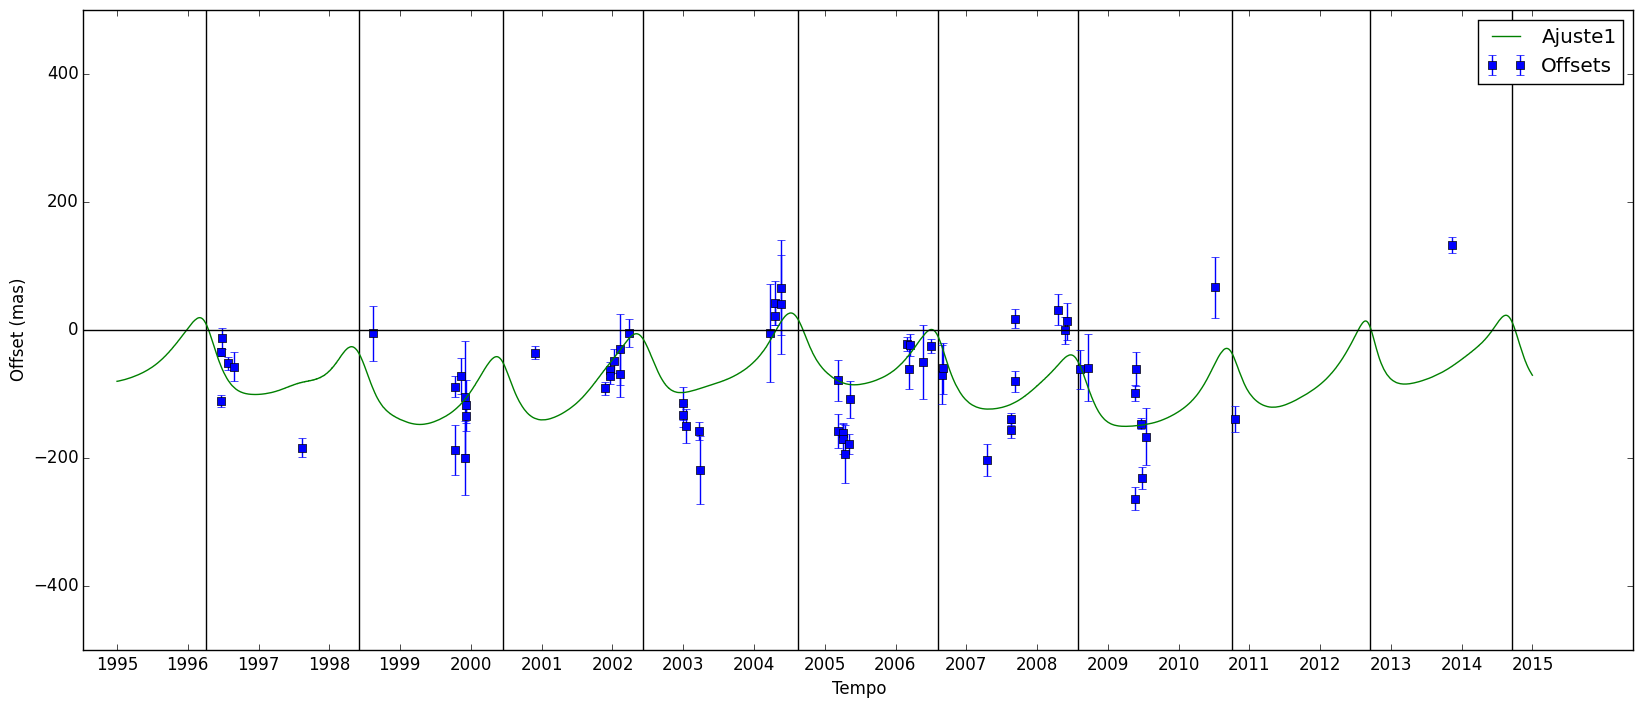
\includegraphics[scale=0.45]{Pasiphae/DEC.png} 
\end{figure}

\begin{figure}[h]
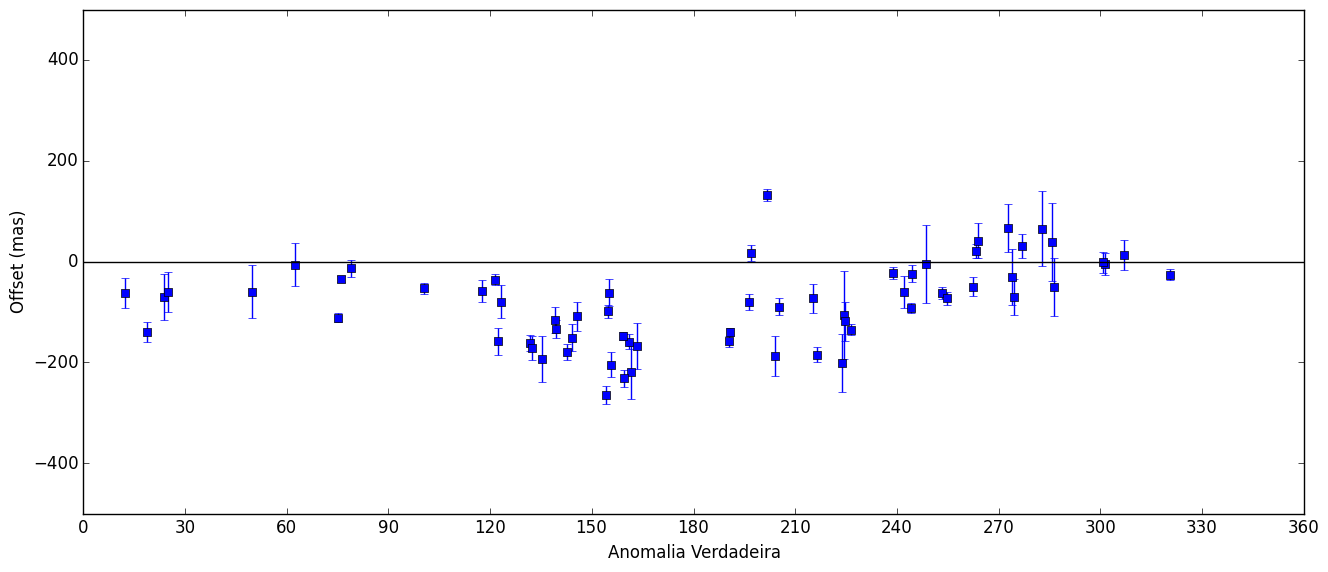
\includegraphics[scale=0.45]{Pasiphae/DEC_anom.png}  
\end{figure}

\begin{table}[h!]
\caption{\label{Tab: Pasiphae-DEC} Resultados dos ajustes para Pasiphae - DEC}
\begin{centering}
\begin{tabular}{cccc}
\hline
\hline
Parâmetro & Com peso & Sem peso & Unidade\tabularnewline
\hline
p[0] & 35 $\pm$ 13 & 26 $\pm$ 10 & mas\\
p[1] & 9 $\pm$ 1 & 8 $\pm$ 2 & anos\\
p[2] & -85 $\pm$ 29 & -110 $\pm$ 45 & graus\\
p[3] & -30 $\pm$ 14 & -48 $\pm$ 11 & mas\\
p[4] & 44 $\pm$ 16 & 58 $\pm$ 13 & mas\\
p[5] & -62 $\pm$ 10 & -67 $\pm$ 9 & mas\\
Residuo & 59 & 60 & mas\\
\hline 
\end{tabular} 
\par\end{centering}
\end{table}

\chapter*{Ananke}

\indent \indent Número total de noites: 30.

\section*{Ascensão Reta}

Foi utilizada a equação \ref{eq:cos}. A equação com seno dava um período de 2 anos

\begin{figure}[h]
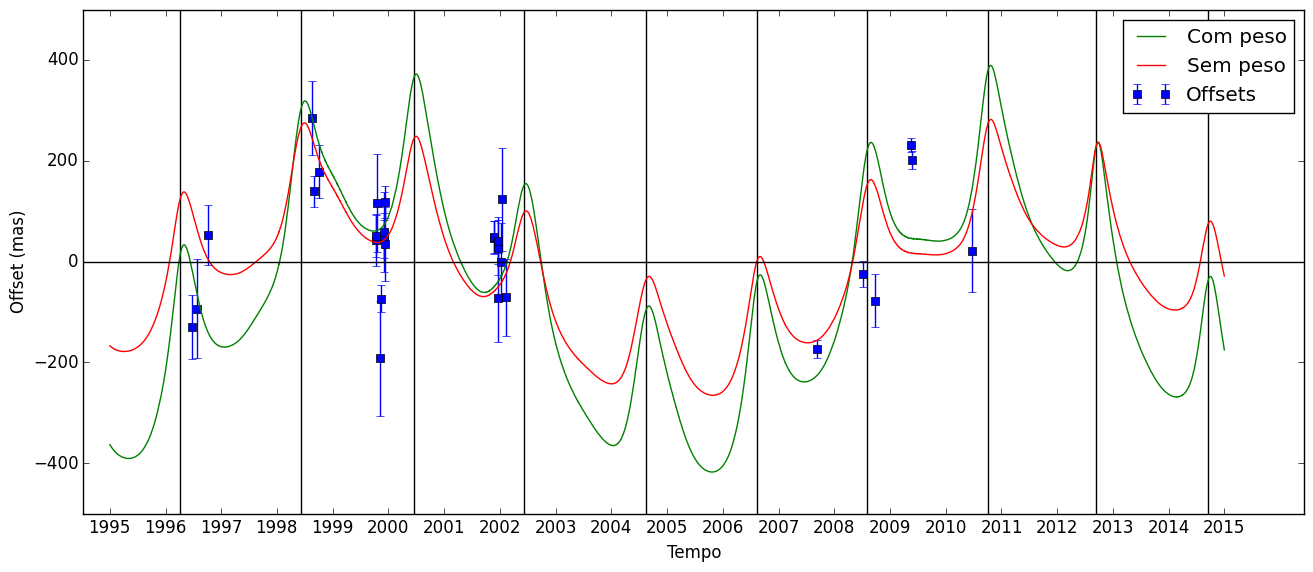
\includegraphics[scale=0.45]{Ananke/RA.png} 
\end{figure}

\begin{figure}[h]
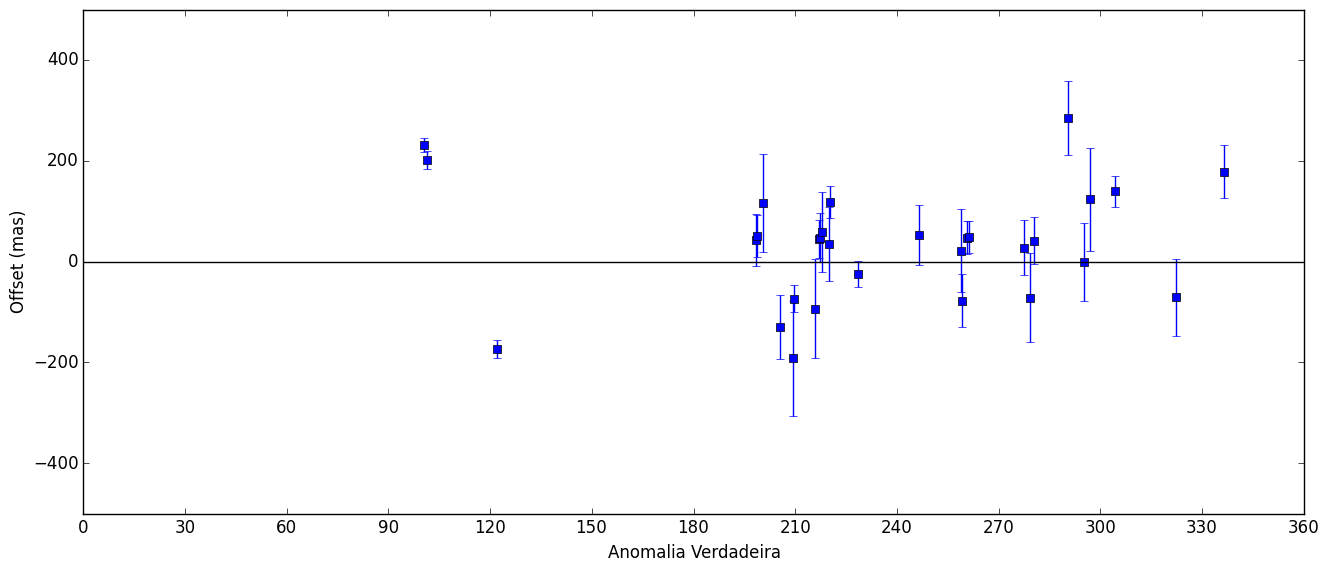
\includegraphics[scale=0.45]{Ananke/RA_anom.png}  
\end{figure}

\begin{table}[h!]
\caption{\label{Tab: Ananke-RA} Resultados dos ajustes para Ananke - RA}
\begin{centering}
\begin{tabular}{cccc}
\hline
\hline
Parâmetro & Com peso & Sem peso & Unidade\tabularnewline
\hline
p[0] & 246 $\pm$ 39 & 160 $\pm$ 43 & mas\\
p[1] & 10.8 $\pm$ 0.5 & 12.0 $\pm$ 0.9 & anos\\
p[2] & 5 $\pm$ 8 & 24 $\pm$ 10 & graus\\
p[3] & 60 $\pm$ 29 & 44 $\pm$ 39 & mas\\
p[4] & 152 $\pm$ 37 & 111 $\pm$ 32 & mas\\
p[5] & -20 $\pm$ 37 & 5 $\pm$ 37 & mas\\
Residuo & 71 & 82 & mas\\
\hline 
\end{tabular} 
\par\end{centering}
\end{table}

\section*{Declinação}

Foi utilizada a equação \ref{eq:cos}. A equação com o seno dava um período de 2 anos

\begin{figure}[h]
\begin{centering}
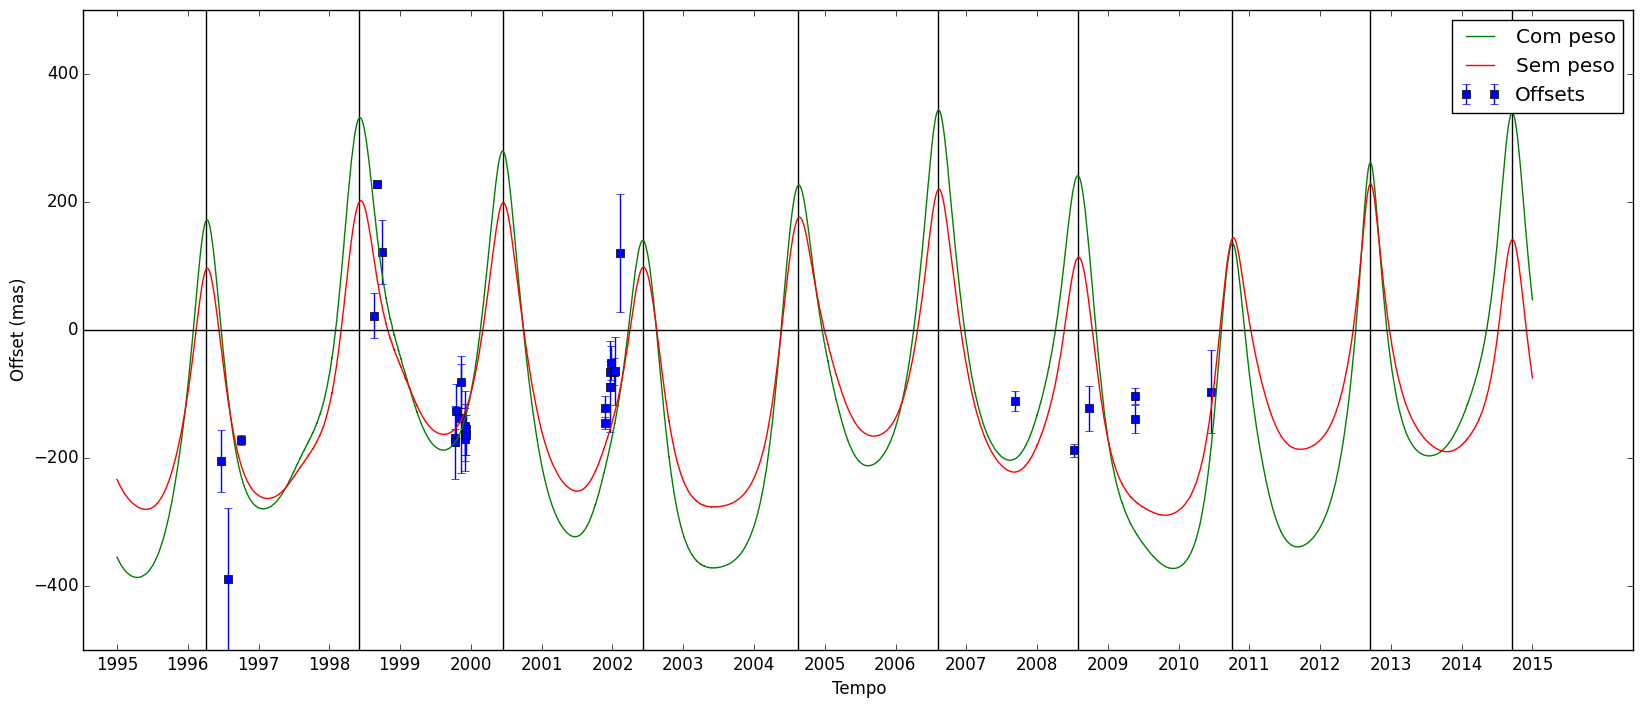
\includegraphics[scale=0.45]{Ananke/DEC.png}
\end{centering}
\end{figure}

\begin{figure}[h]
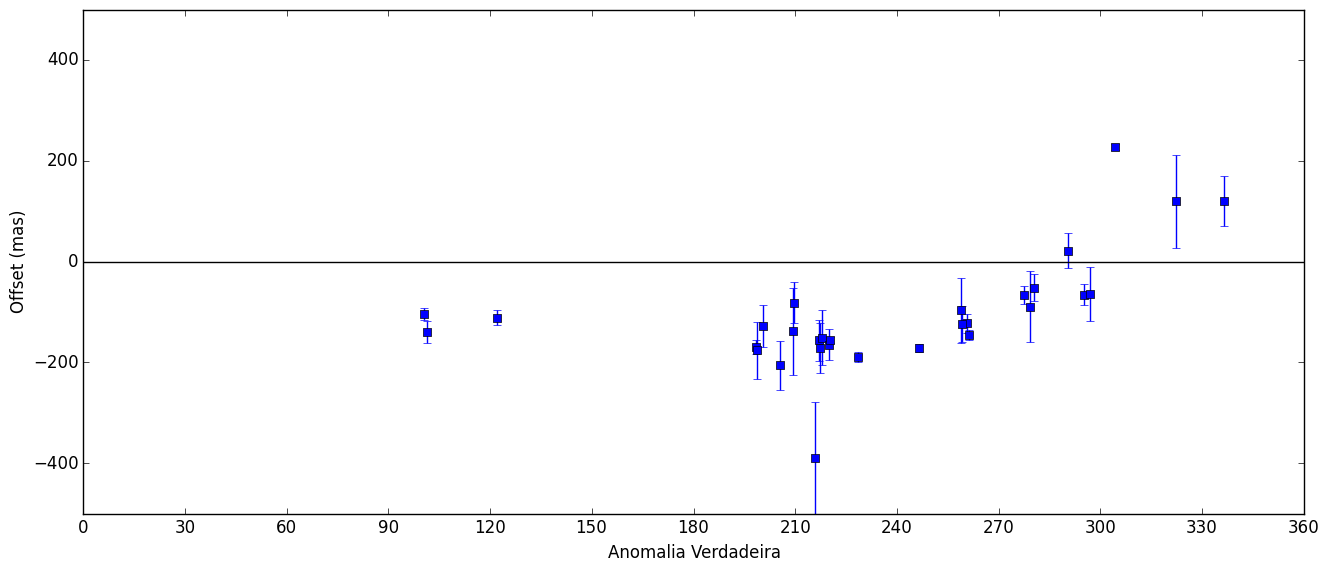
\includegraphics[scale=0.45]{Ananke/DEC_anom.png}  
\end{figure}

\begin{table}[h!]
\caption{\label{Tab: Ananke-DEC} Resultados dos ajustes para Ananke - DEC}
\begin{centering}
\begin{tabular}{cccc}
\hline
\hline
Parâmetro & Com peso & Sem peso & Unidade\tabularnewline
\hline
p[0] & 105 $\pm$ 8 & 66 $\pm$ 12 & mas\\
p[1] & 7.6 $\pm$ 0.2 & 6.6 $\pm$ 0.4 & anos\\
p[2] & 45 $\pm$ 5 & 31 $\pm$ 18 & graus\\
p[3] & 9 $\pm$ 11 & 18 $\pm$ 18 & mas\\
p[4] & 260 $\pm$ 10 & 194 $\pm$ 19 & mas\\
p[5] & -22 $\pm$ 13 & -34 $\pm$ 16 & mas\\
Residuo & 23 & 46 & mas\\
\hline 
\end{tabular} 
\par\end{centering}
\end{table}

\chapter*{Carme}

\indent \indent Número total de noites: 44.

\section*{Ascensão Reta}

Foi utilizada a equação \ref{eq:cos}. A equação com o seno não conseguia ajustar bem o período do tempo com o peso. encontrava 33 $\pm$ 43.

\begin{figure}[h]
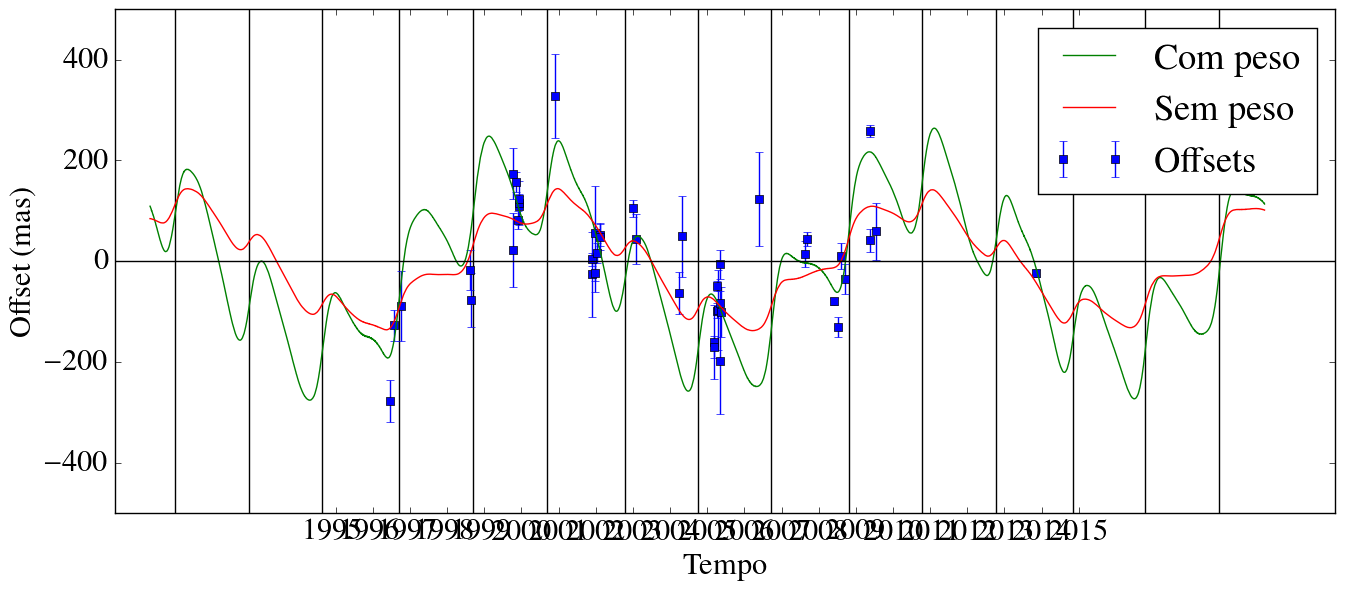
\includegraphics[scale=0.45]{Carme/RA.png} 
\end{figure}

\begin{figure}[h]
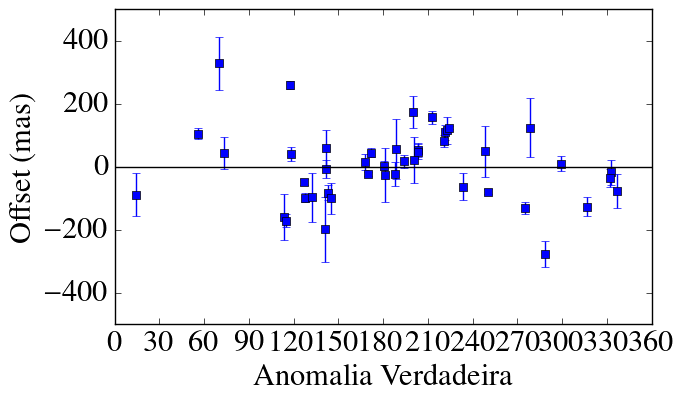
\includegraphics[scale=0.45]{Carme/RA_anom.png}  
\end{figure}

\begin{table}[h!]
\caption{\label{Tab: Carme-RA} Resultados dos ajustes para Carme - RA}
\begin{centering}
\begin{tabular}{cccc}
\hline
\hline
Parâmetro & Com peso & Sem peso & Unidade\tabularnewline
\hline
p[0] & 167 $\pm$ 14 & 112 $\pm$ 20 & mas\\
p[1] & 10.7 $\pm$ 0.2 & 9.9 $\pm$ 0.7 & anos\\
p[2] & 1 $\pm$ 8 & -24 $\pm$ 16 & graus\\
p[3] & 104 $\pm$ 16 & 33 $\pm$ 22 & mas\\
p[4] & -17 $\pm$ 20 & 0 $\pm$ 24 & mas\\
p[5] & -4 $\pm$ 15 & 0 $\pm$ 17 & mas\\
Residuo & 45 & 83 & mas\\
\hline 
\end{tabular} 
\par\end{centering}
\end{table}

\section*{Declinação}

Foi utilizada a equação \ref{eq:linear}.

\begin{figure}[h]
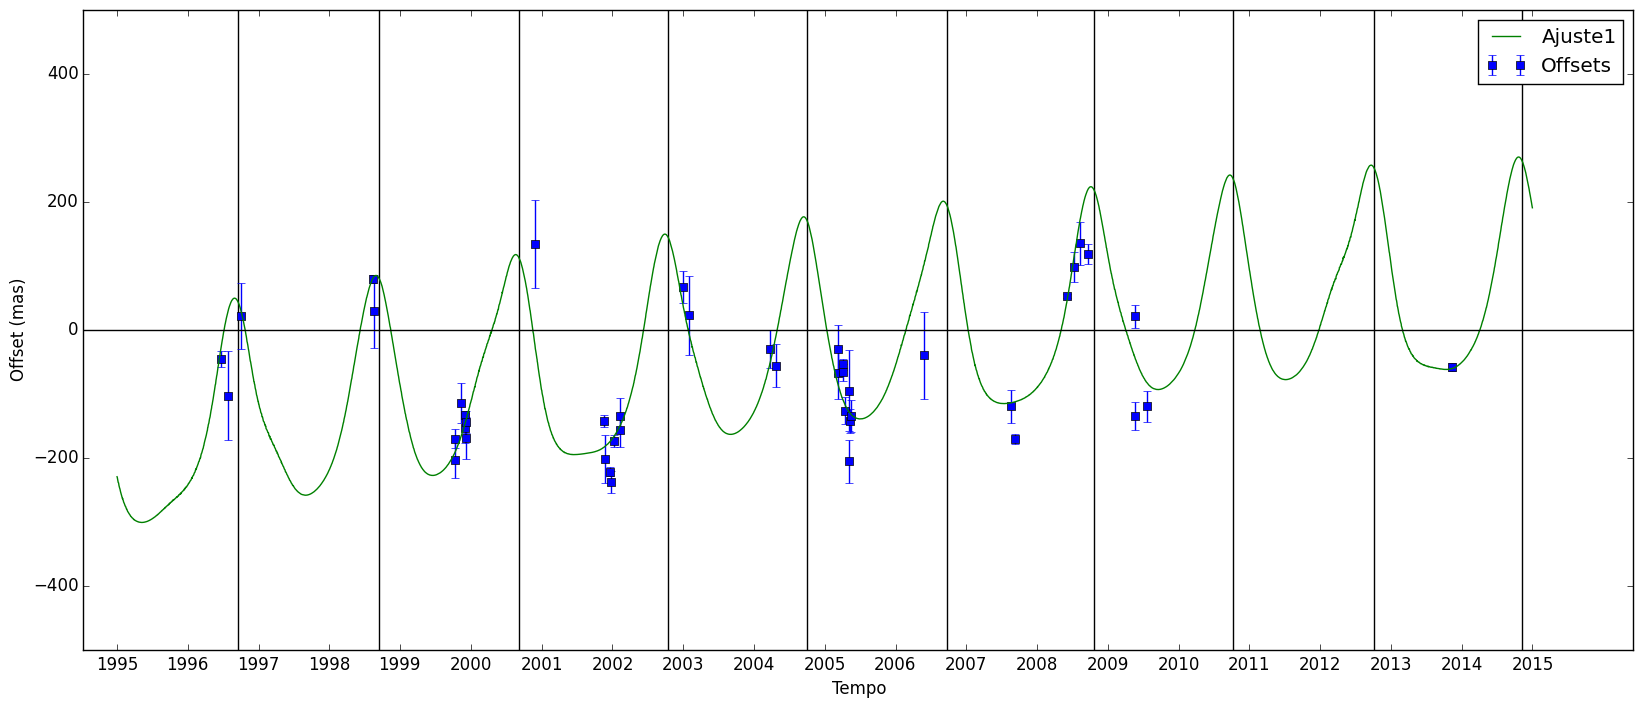
\includegraphics[scale=0.45]{Carme/DEC.png} 
\end{figure}

\begin{figure}[h]
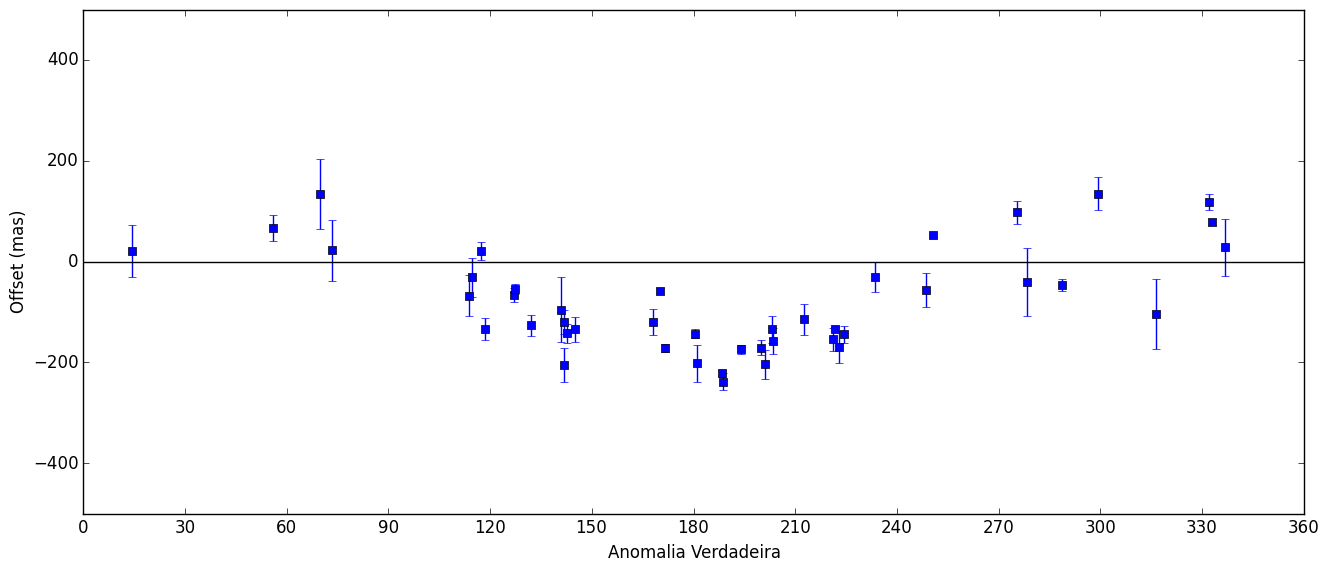
\includegraphics[scale=0.45]{Carme/DEC_anom.png}  
\end{figure}

\begin{table}[h!]
\caption{\label{Tab: Carme-DEC} Resultados dos ajustes para Carme - DEC}
\begin{centering}
\begin{tabular}{cccc}
\hline
\hline
Parâmetro & Com peso & Sem peso & Unidade\tabularnewline
\hline
p[0] & 12 $\pm$ 1 & 10 $\pm$ 2 & mas/ano\\
p[1] & -44 $\pm$ 9 & -4 $\pm$ 12 & mas\\
p[2] & 155 $\pm$ 9 & 140 $\pm$ 12 & mas\\
p[3] & -55 $\pm$ 9 & -57 $\pm$ 11 & mas\\
Residuo & 29 & 47 & mas\\
\hline 
\end{tabular} 
\par\end{centering}
\end{table}

\chapter*{Elara}

\indent \indent Número total de noites: 65.

\section*{Ascensão Reta}

Foi utilizada a equação \ref{eq:sin}

\begin{figure}[h]
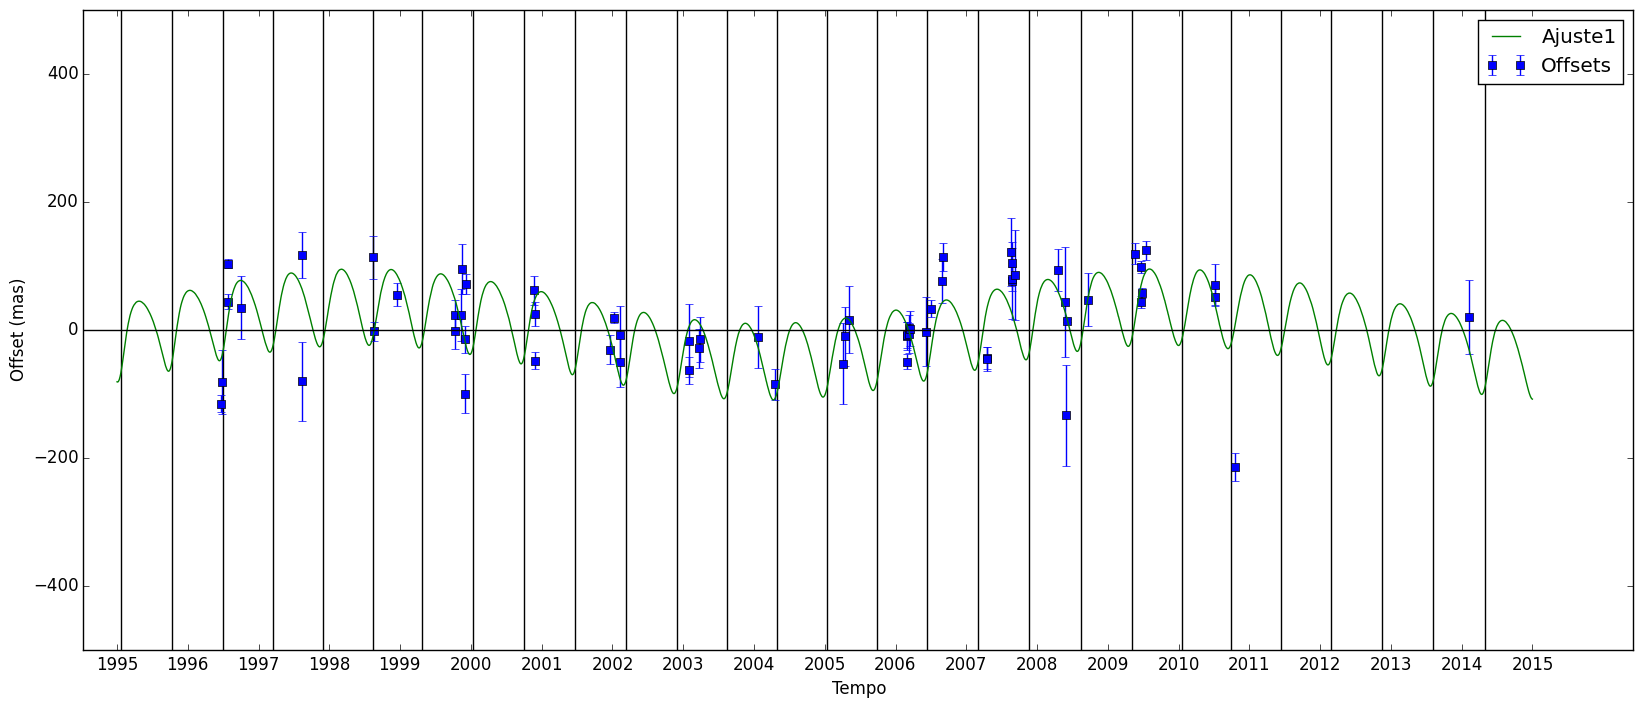
\includegraphics[scale=0.45]{Elara/RA.png} 
\end{figure}

\begin{figure}[h]
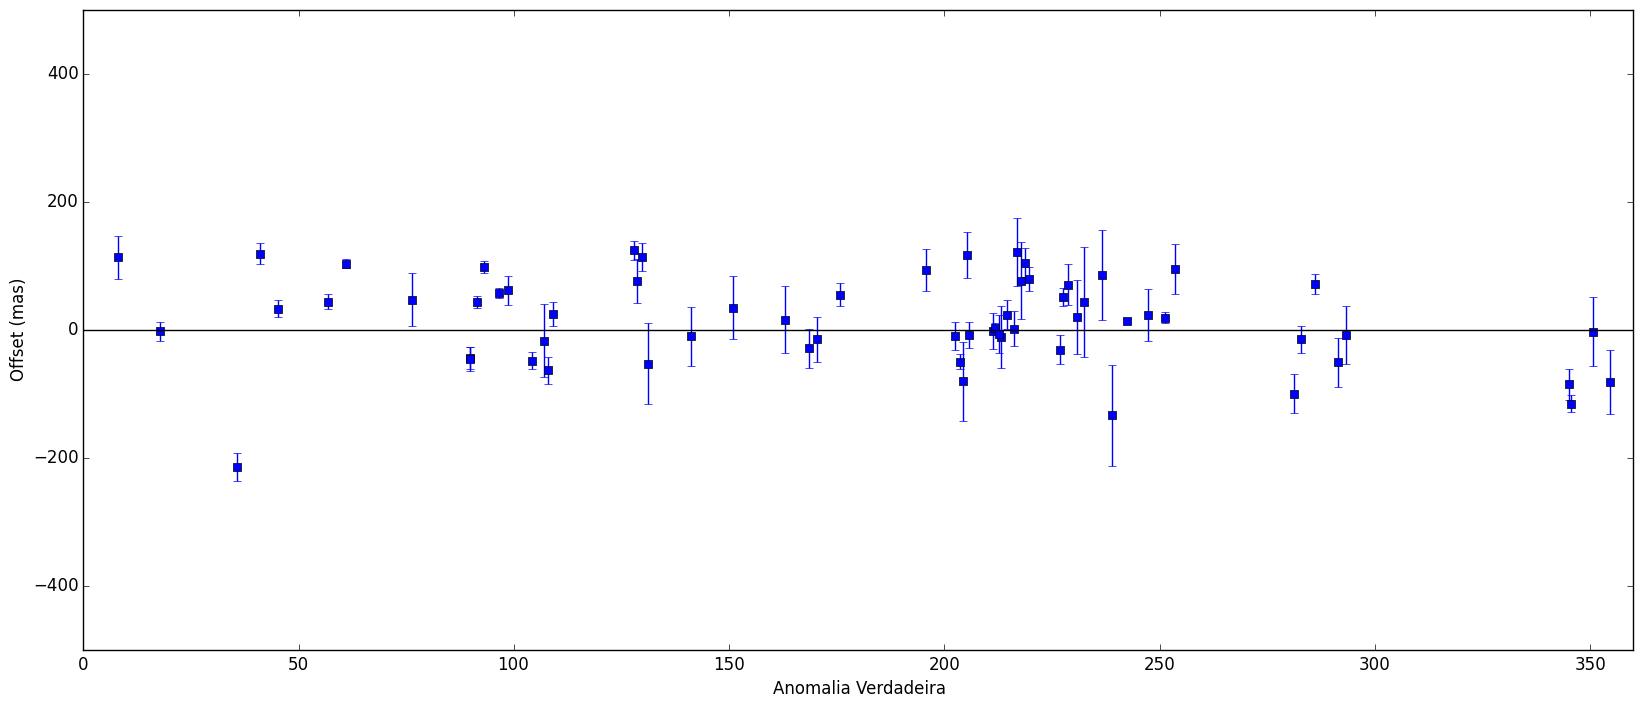
\includegraphics[scale=0.45]{Elara/RA_anom.png}  
\end{figure}

\begin{table}[h!]
\caption{\label{Tab: Elara-RA} Resultados dos ajustes para Elara - RA}
\begin{centering}
\begin{tabular}{cccc}
\hline
\hline
Parâmetro & Com peso & Sem peso & Unidade\tabularnewline
\hline
p[0] & -42 $\pm$ 17 & -63 $\pm$ 20 & mas\\
p[1] & 11 $\pm$ 2 & 8.5 $\pm$ 0.8 & anos\\
p[2] & -41 $\pm$ 26 & -82 $\pm$ 24 & graus\\
p[3] & 33 $\pm$ 13 & 27 $\pm$ 18 & mas\\
p[4] & -49 $\pm$ 23 & -57 $\pm$ 21 & mas\\
p[5] & -7 $\pm$ 14 & -23 $\pm$ 15 & mas\\
Residuo & 66 & 98 & mas\\
\hline 
\end{tabular} 
\par\end{centering}
\end{table}

\section*{Declinação}

Foi utilizada a equação \ref{eq:sin}.

\begin{figure}[h]
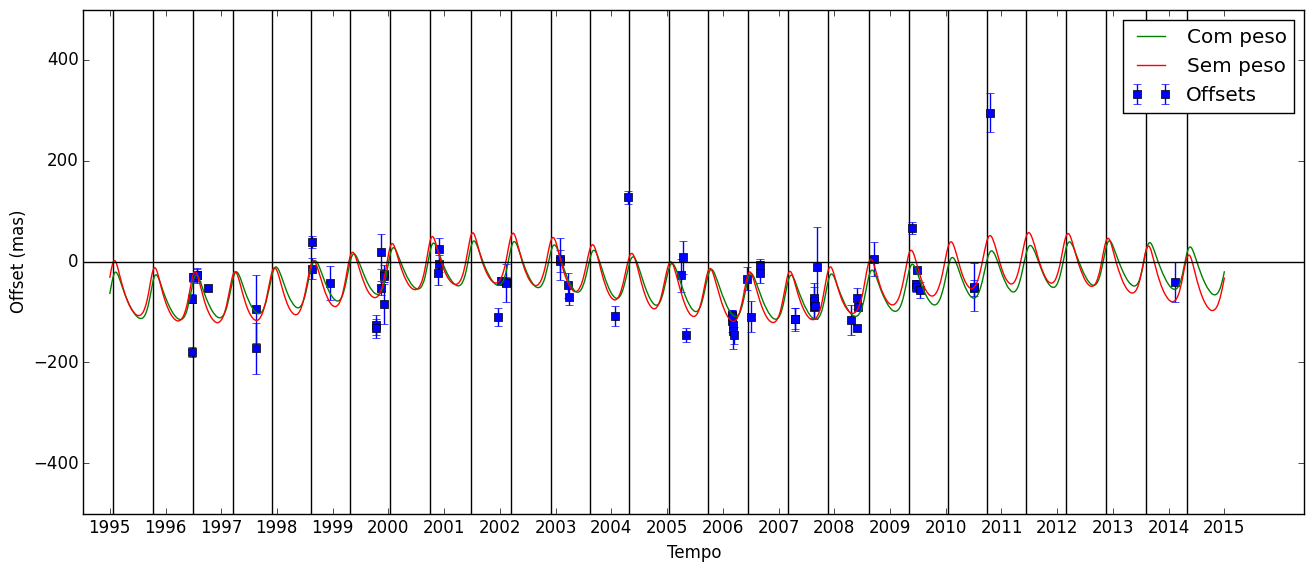
\includegraphics[scale=0.45]{Elara/DEC.png} 
\end{figure}

\begin{figure}[h]
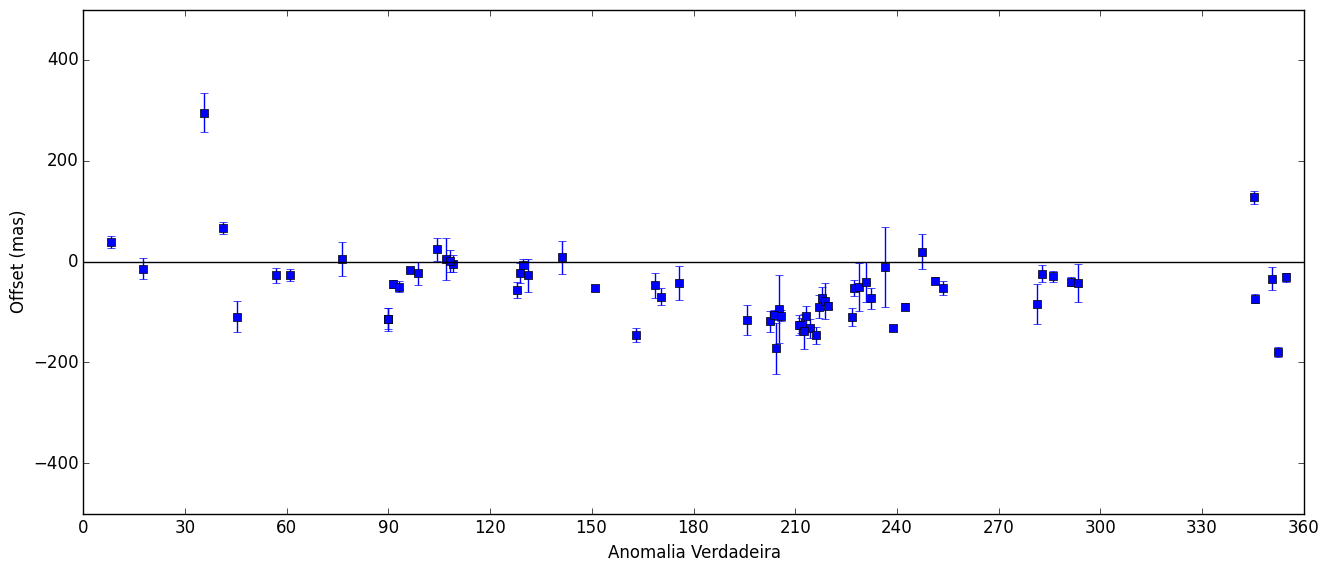
\includegraphics[scale=0.45]{Elara/DEC_anom.png}  
\end{figure}

\begin{table}[h!]
\caption{\label{Tab: Elara-DEC} Resultados dos ajustes para Elara - DEC}
\begin{centering}
\begin{tabular}{cccc}
\hline
\hline
Parâmetro & Com peso & Sem peso & Unidade\tabularnewline
\hline
p[0] & 34 $\pm$ 8 & 39 $\pm$ 10 & mas\\
p[1] & 11.1 $\pm$ 1.2 & 9.8 $\pm$ 0.9 & anos\\
p[2] & 33 $\pm$ 27 & 23 $\pm$ 24 & graus\\
p[3] & 32 $\pm$ 8 & 26 $\pm$ 10 & mas\\
p[4] & 29 $\pm$ 8 & 42 $\pm$ 11 & mas\\
p[5] & -37 $\pm$ 7 & -31 $\pm$ 8 & mas\\
Residuo & 41 & 55 & mas\\
\hline 
\end{tabular} 
\par\end{centering}
\end{table}

\chapter*{Himalia}

\indent \indent Número total de noites: 98.

\section*{Ascensão Reta}

Foi utilizada a equação \ref{eq:sin}.

\begin{figure}[h]
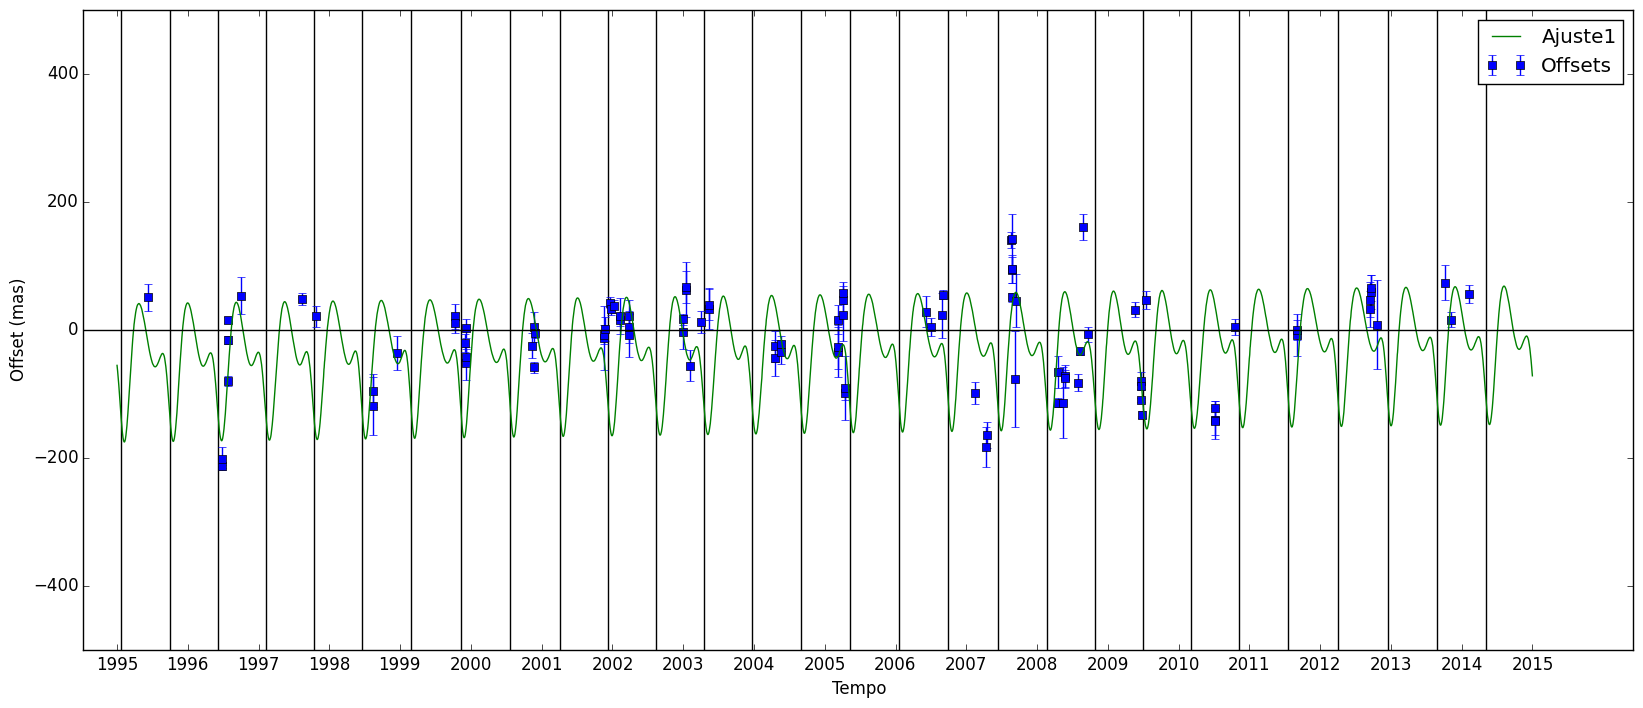
\includegraphics[scale=0.45]{Himalia/RA.png} 
\end{figure}

\begin{figure}[h]
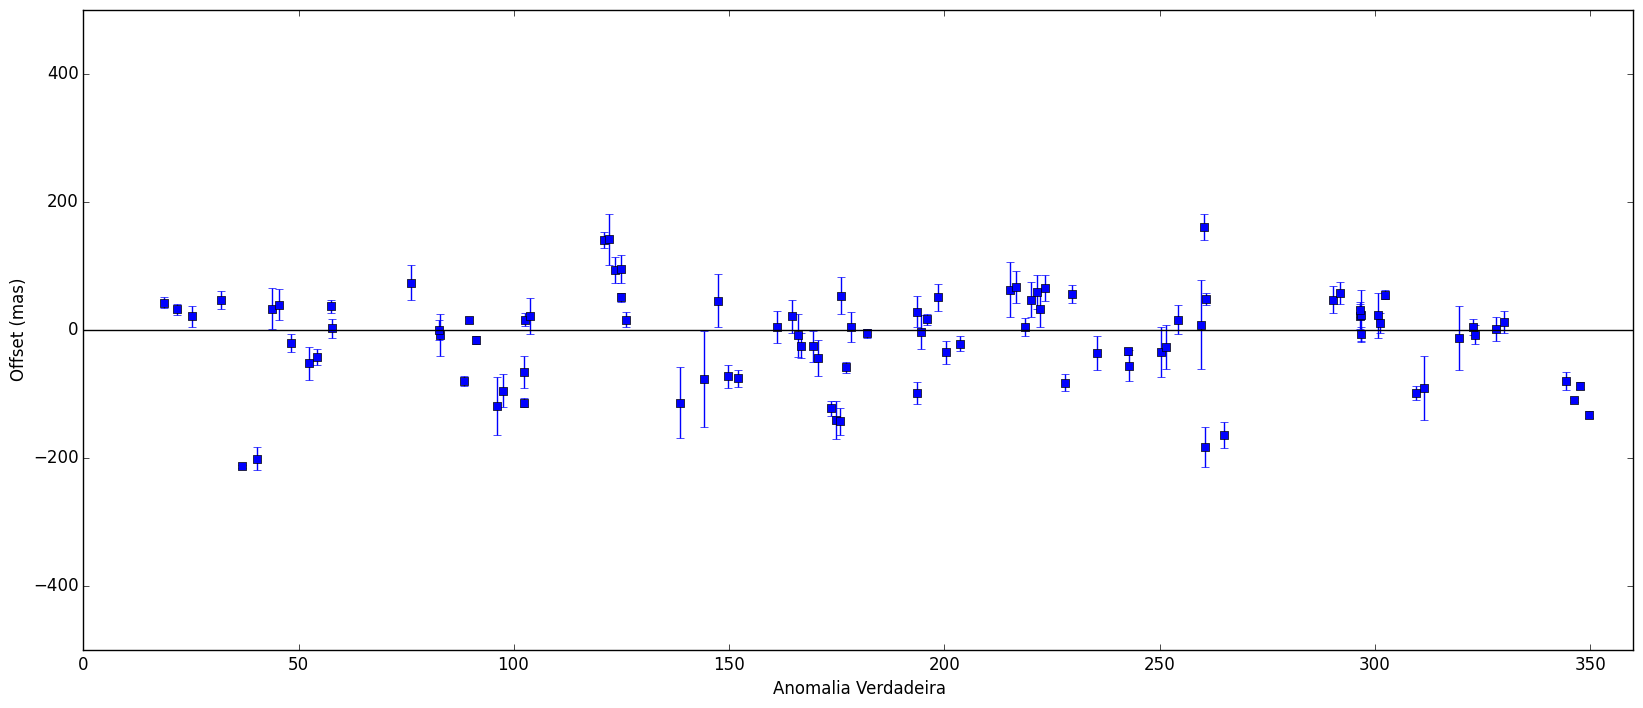
\includegraphics[scale=0.45]{Himalia/RA_anom.png}  
\end{figure}

\begin{table}[h!]
\caption{\label{Tab: Himalia-RA} Resultados dos ajustes para Himalia - RA}
\begin{centering}
\begin{tabular}{cccc}
\hline
\hline
Parâmetro & Com peso & Sem peso & Unidade\tabularnewline
\hline
p[0] & 71 $\pm$ 24 & 49 $\pm$ 19 & mas\\
p[1] & 18 $\pm$ 8 & 12 $\pm$ 2 & anos\\
p[2] & 5 $\pm$ 46 & 12 $\pm$ 41 & graus\\
p[3] & 0 $\pm$ 21 & -17 $\pm$ 21 & mas\\
p[4] & -55 $\pm$ 17 & -36 $\pm$ 21 & mas\\
p[5] & -49 $\pm$ 36 & -32 $\pm$ 14 & mas\\
Residuo & 108 & 136 & mas\\
\hline 
\end{tabular} 
\par\end{centering}
\end{table}

\section*{Declinação}

Foi utilizada a equação \ref{eq:sin}.

\begin{figure}[h]
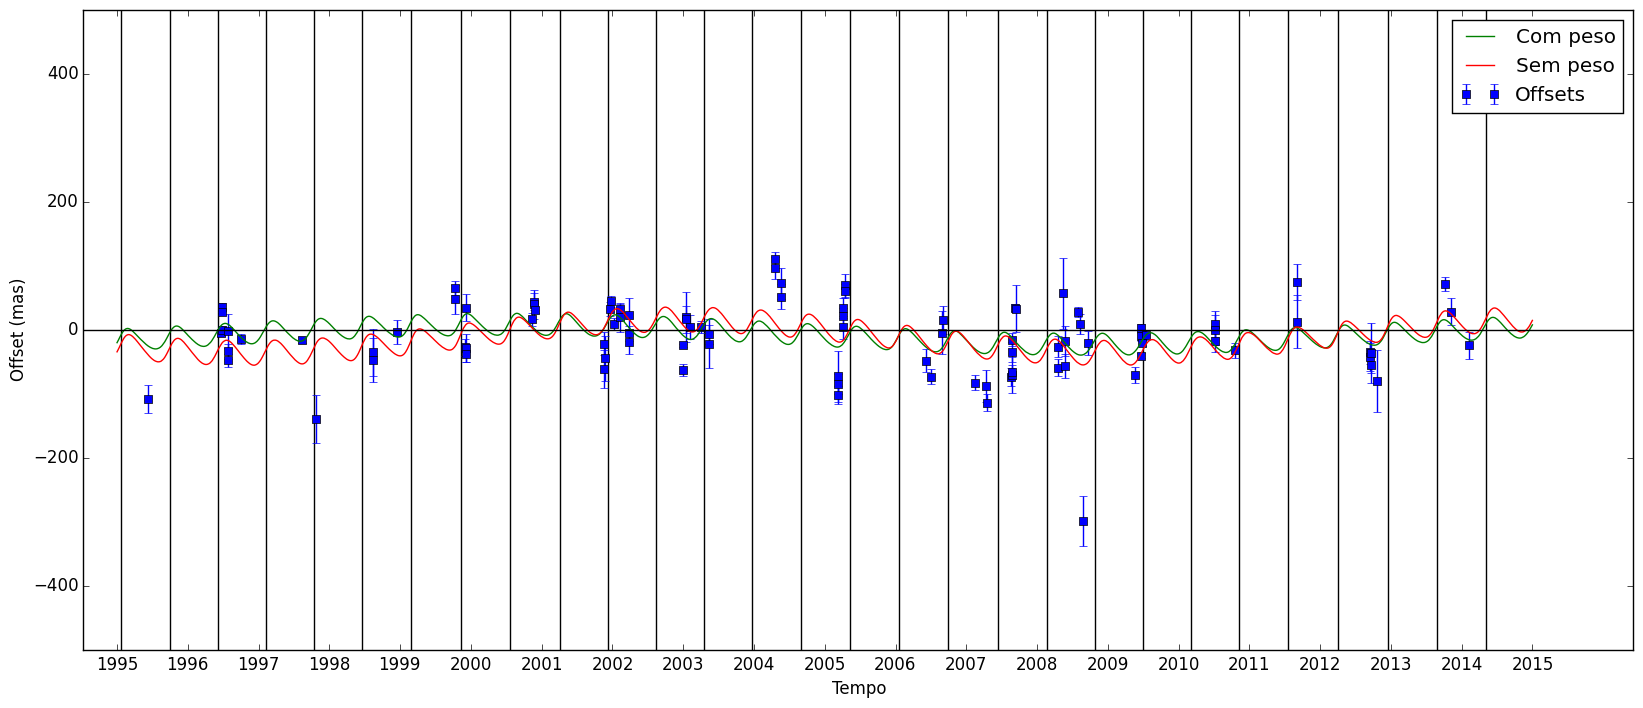
\includegraphics[scale=0.45]{Himalia/DEC.png} 
\end{figure}

\begin{figure}[h]
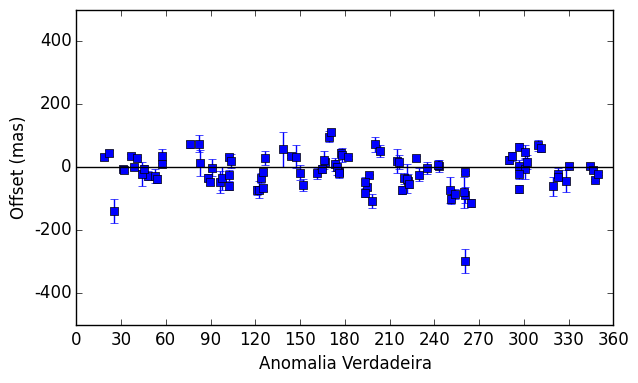
\includegraphics[scale=0.45]{Himalia/DEC_anom.png}  
\end{figure}

\begin{table}[h!]
\caption{\label{Tab: Himalia-DEC} Resultados dos ajustes para Himalia - DEC}
\begin{centering}
\begin{tabular}{cccc}
\hline
\hline
Parâmetro & Com peso & Sem peso & Unidade\tabularnewline
\hline
p[0] & 15 $\pm$ 5 & 26 $\pm$ 7 & mas\\
p[1] & 16 $\pm$ 3 & 12.2 $\pm$ 1.6 & anos\\
p[2] & 76 $\pm$ 23 & 3 $\pm$ 29 & graus\\
p[3] & 15 $\pm$ 6 & 19 $\pm$ 8 & mas\\
p[4] & 7 $\pm$ 5 & 3 $\pm$ 7 & mas\\
p[5] & -7 $\pm$ 4 & -10 $\pm$ 5 & mas\\
Residuo & 34 & 51 & mas\\
\hline 
\end{tabular} 
\par\end{centering}
\end{table}

\chapter*{Lysithea}

\indent \indent Número total de noites: 29.

\section*{Ascensão Reta}

Foi utilizada a equação \ref{eq:cos}. A equação com o seno diverge muito com período de mais de 400 anos no tempo para o ajuste com peso.

\begin{figure}[h]
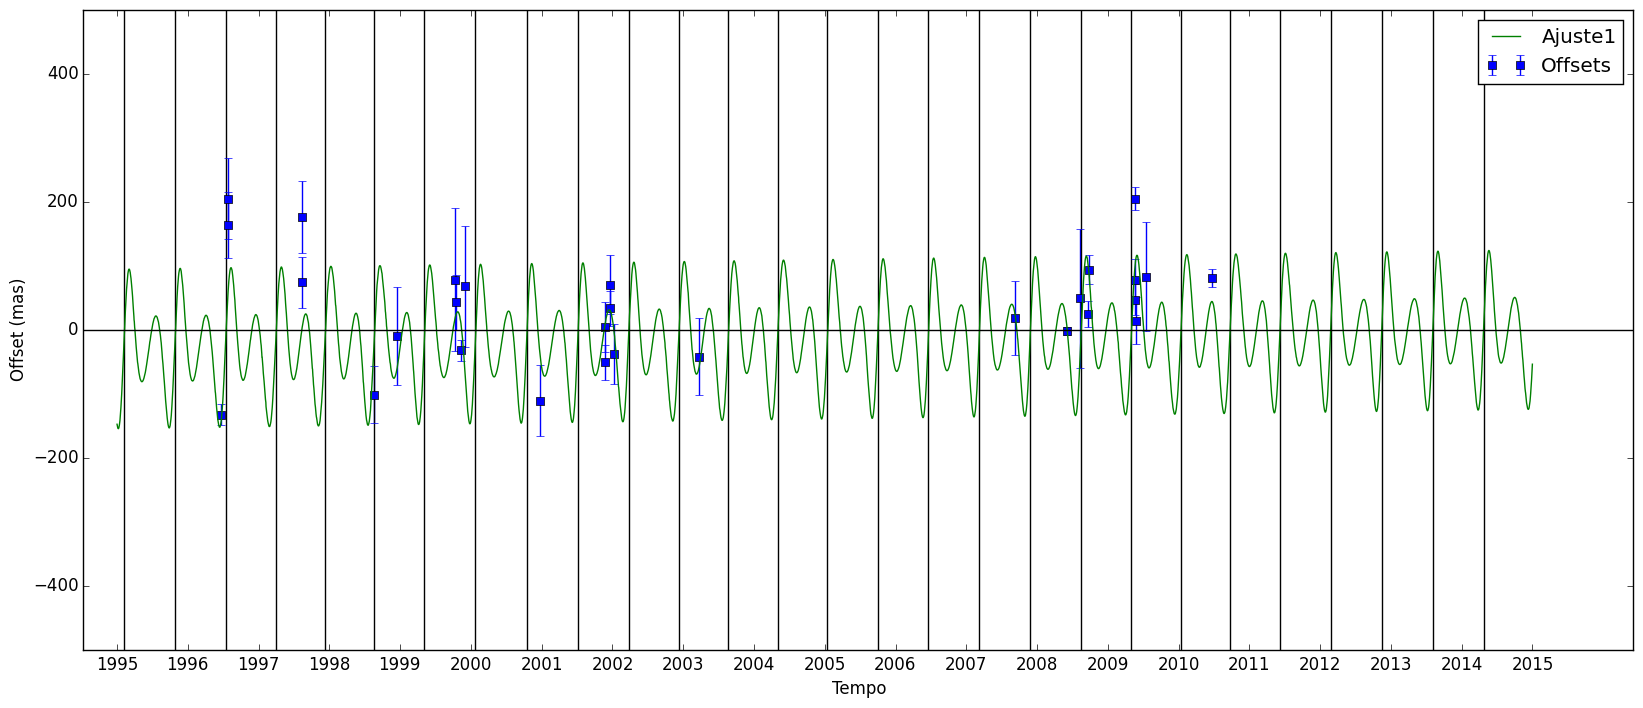
\includegraphics[scale=0.45]{Lysithea/RA.png} 
\end{figure}

\begin{figure}[h]
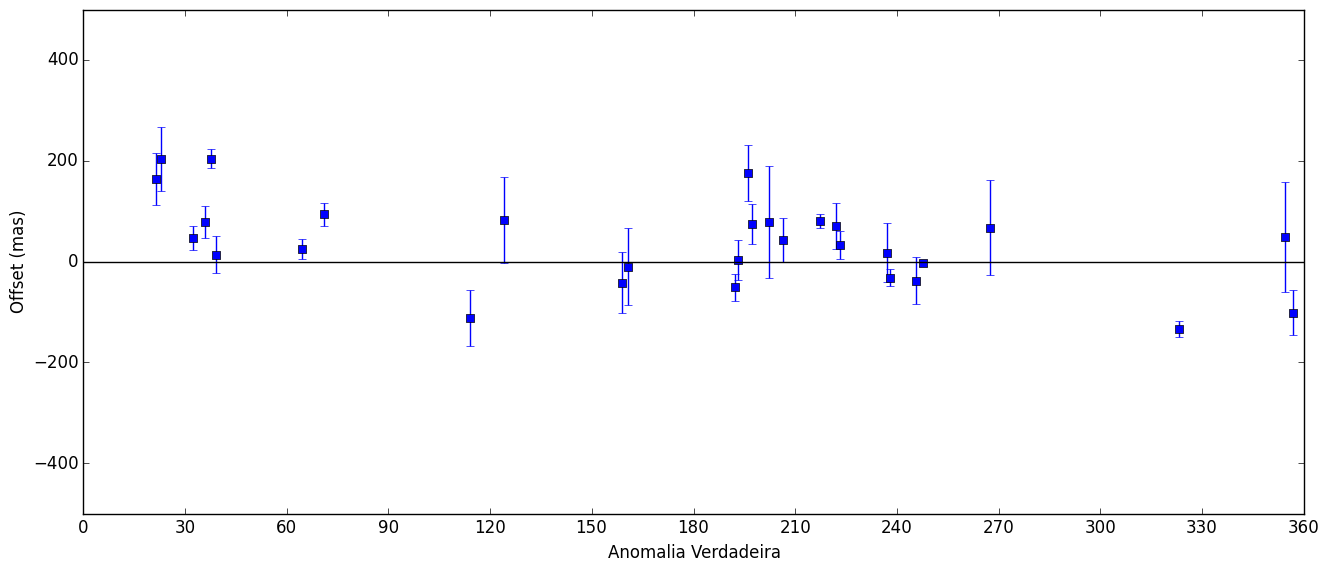
\includegraphics[scale=0.45]{Lysithea/RA_anom.png}  
\end{figure}

\begin{table}[h!]
\caption{\label{Tab: Lysithea-RA} Resultados dos ajustes para Lysithea - RA}
\begin{centering}
\begin{tabular}{cccc}
\hline
\hline
Parâmetro & Com peso & Sem peso & Unidade\tabularnewline
\hline
p[0] & 88 $\pm$ 37 & 117 $\pm$ 350 & mas\\
p[1] & 10.8 $\pm$ 0.9 & 24 $\pm$ 49 & anos\\
p[2] & 31 $\pm$ 21 & 132 $\pm$ 96 & graus\\
p[3] & 67 $\pm$ 27 & 12 $\pm$ 28 & mas\\
p[4] & -38 $\pm$ 33 & -24 $\pm$ 26 & mas\\
p[5] & -16 $\pm$ 28 & 79 $\pm$ 370 & mas\\
Residuo & 54 & 73 & mas\\
\hline 
\end{tabular} 
\par\end{centering}
\end{table}

\section*{Declinação}

Foi utilizada a equação \ref{eq:sin}.

\begin{figure}[h]
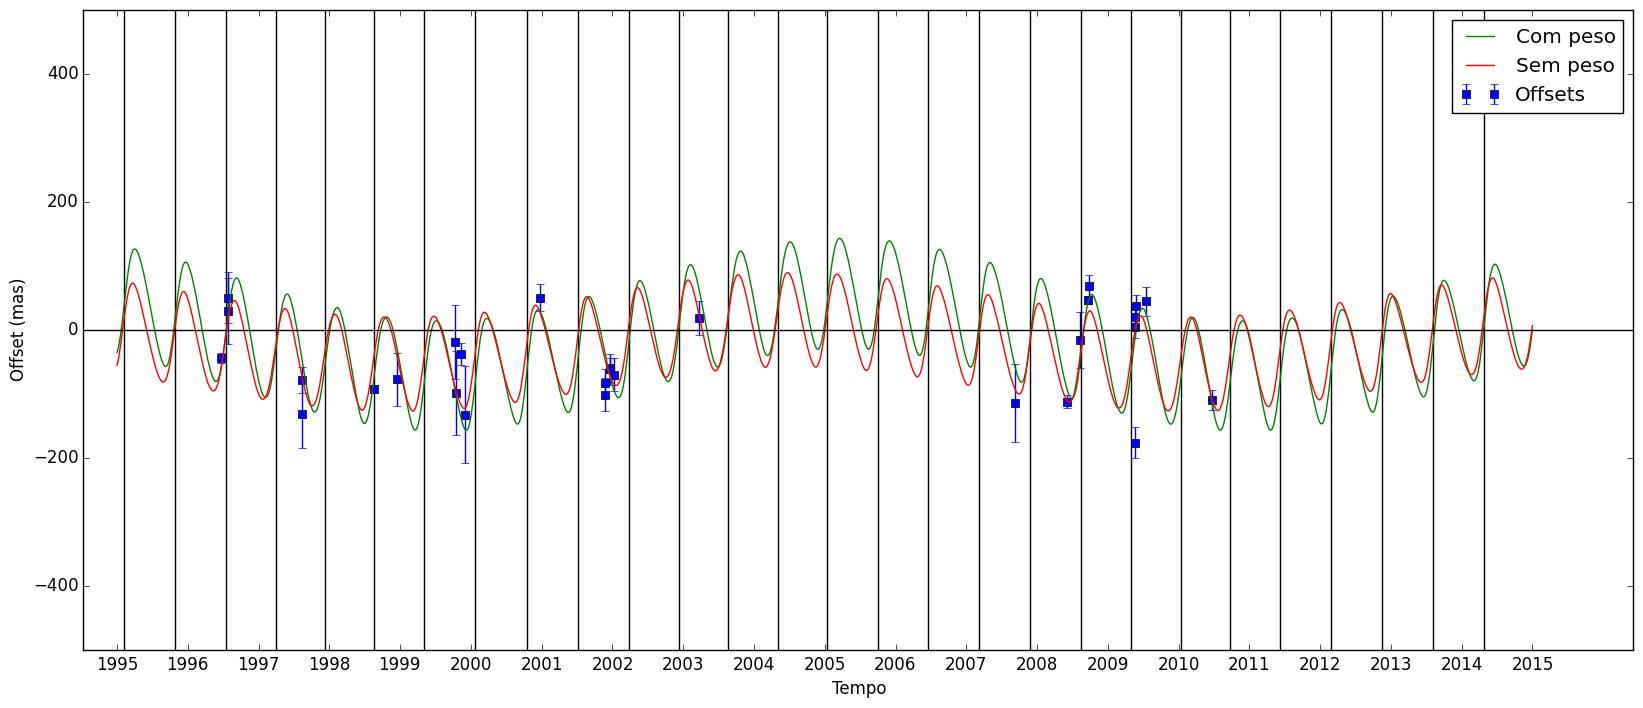
\includegraphics[scale=0.45]{Lysithea/DEC.png} 
\end{figure}

\begin{figure}[h]
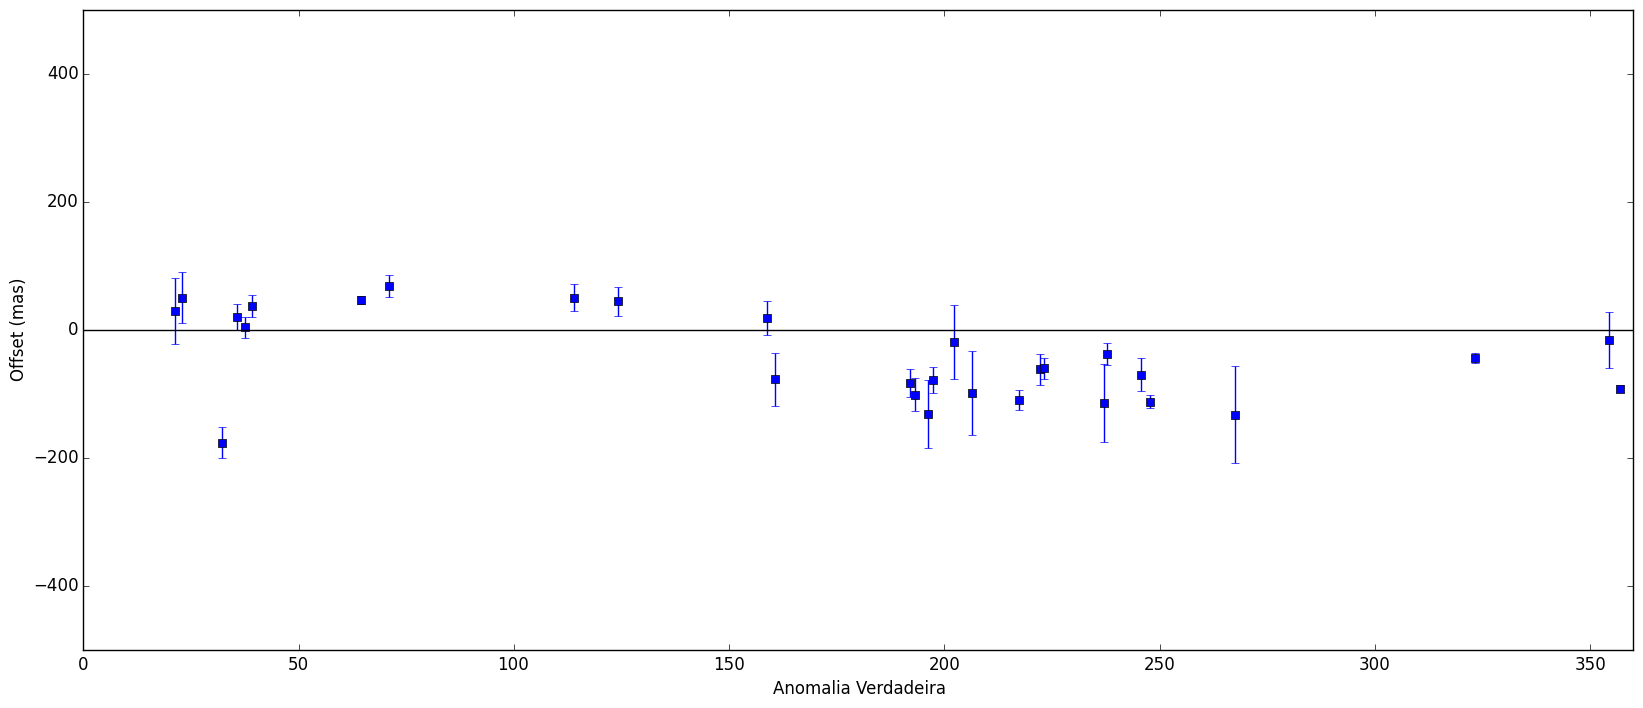
\includegraphics[scale=0.45]{Lysithea/DEC_anom.png}  
\end{figure}

\begin{table}[h!]
\caption{\label{Tab: Lysithea-DEC} Resultados dos ajustes para Lysithea - DEC}
\begin{centering}
\begin{tabular}{cccc}
\hline
\hline
Parâmetro & Com peso & Sem peso & Unidade\tabularnewline
\hline
p[0] & 64 $\pm$ 20 & 34 $\pm$ 24 & mas\\
p[1] & 11.3 $\pm$ 0.7 & 11.1 $\pm$ 1.9 & anos\\
p[2] & -77 $\pm$ 16 & -57 $\pm$ 29 & graus\\
p[3] & 85 $\pm$ 14 & 72 $\pm$ 17 & mas\\
p[4] & -12 $\pm$ 15 & 11 $\pm$ 16 & mas\\
p[5] & -8 $\pm$ 14 & -19 $\pm$ 15 & mas\\
Residuo & 32 & 46 & mas\\
\hline 
\end{tabular} 
\par\end{centering}
\end{table}

\chapter*{Phoebe}

\indent \indent Número total de noites: 133.

\section*{Ascensão Reta}

Foi utilizada a equação \ref{eq:sin}

\begin{figure}[h]
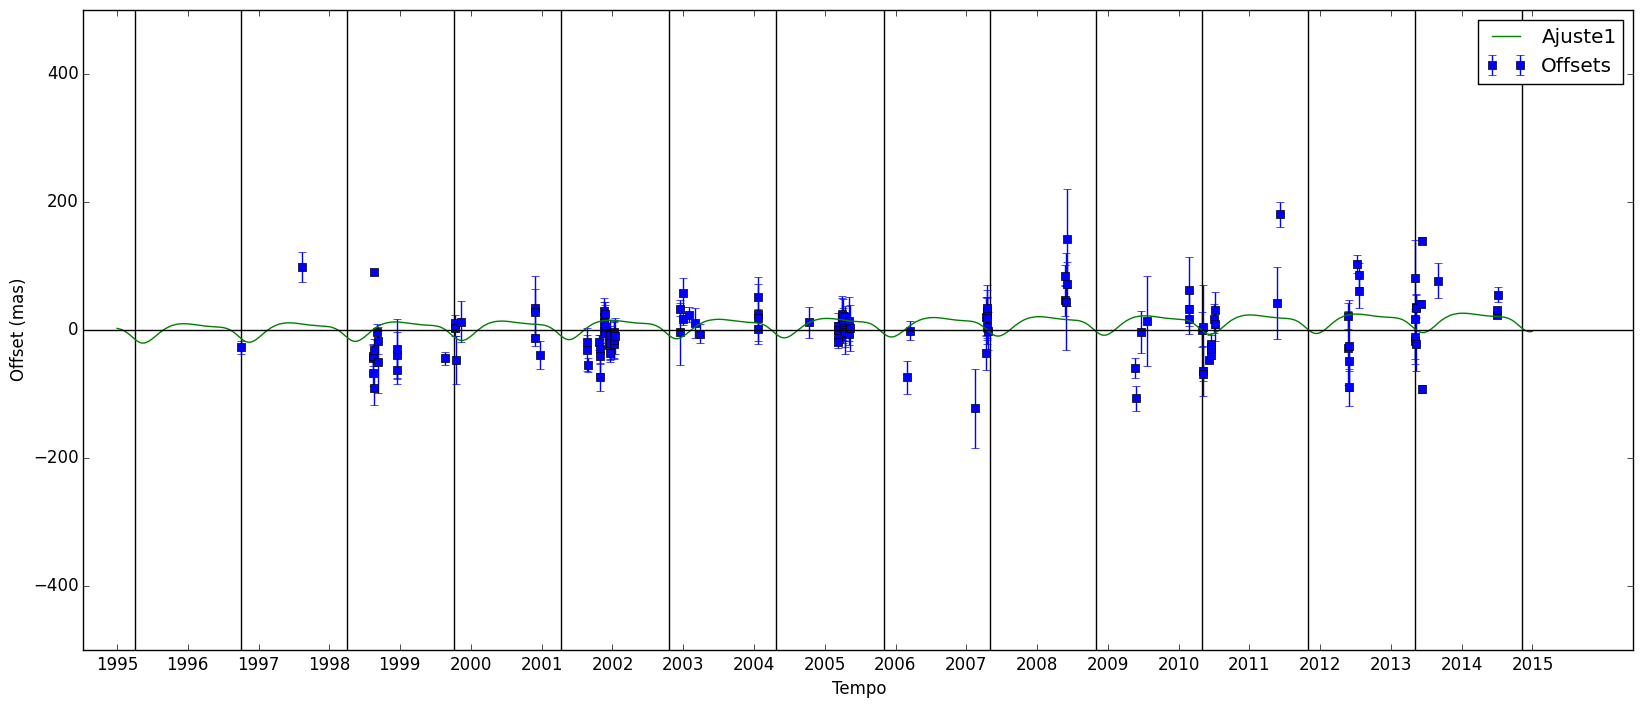
\includegraphics[scale=0.45]{Phoebe/RA.png} 
\end{figure}

\begin{figure}[h]
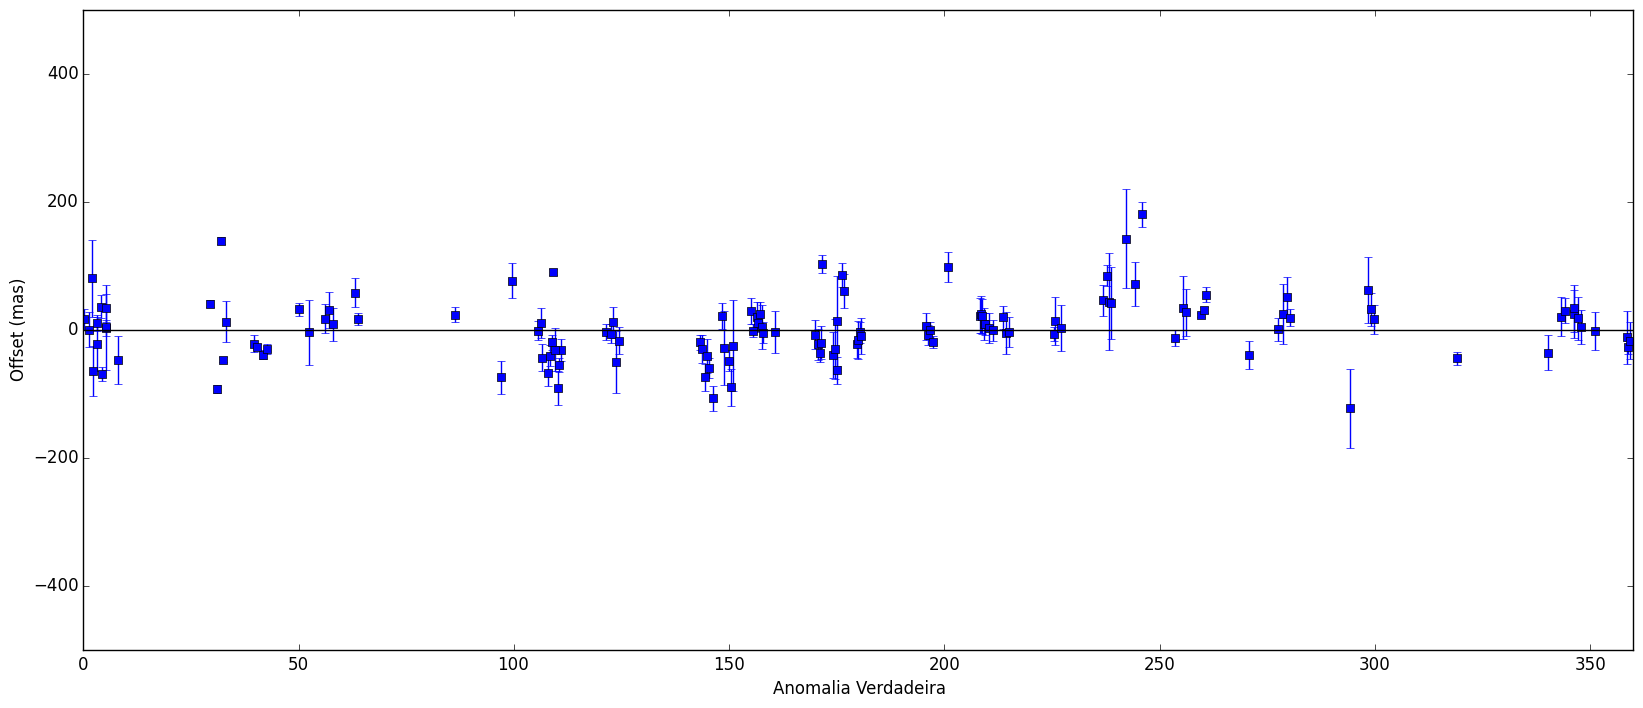
\includegraphics[scale=0.45]{Phoebe/RA_anom.png}  
\end{figure}

\begin{table}[h!]
\caption{\label{Tab: Phoebe-RA} Resultados dos ajustes para Phoebe - RA}
\begin{centering}
\begin{tabular}{cccc}
\hline
\hline
Parâmetro & Com peso & Sem peso & Unidade\tabularnewline
\hline
p[0] & -17 $\pm$ 8 & -17 $\pm$ 8 & mas\\
p[1] & 0.99 $\pm$ 0.01 & 1.01 $\pm$ 0.01 & anos\\
p[2] & 36 $\pm$ 49 & 112 $\pm$ 31 & graus\\
p[3] & -8 $\pm$ 7 & -26 $\pm$ 6 & mas\\
p[4] & -12 $\pm$ 8 & 1 $\pm$ 5 & mas\\
p[5] & 2 $\pm$ 9 & 8 $\pm$ 8 & mas\\
Residuo & 49 & 43 & mas\\
\hline 
\end{tabular} 
\par\end{centering}
\end{table}

\section*{Declinação}

Foi utilizada a equação \ref{eq:sin}.

\begin{figure}[h]
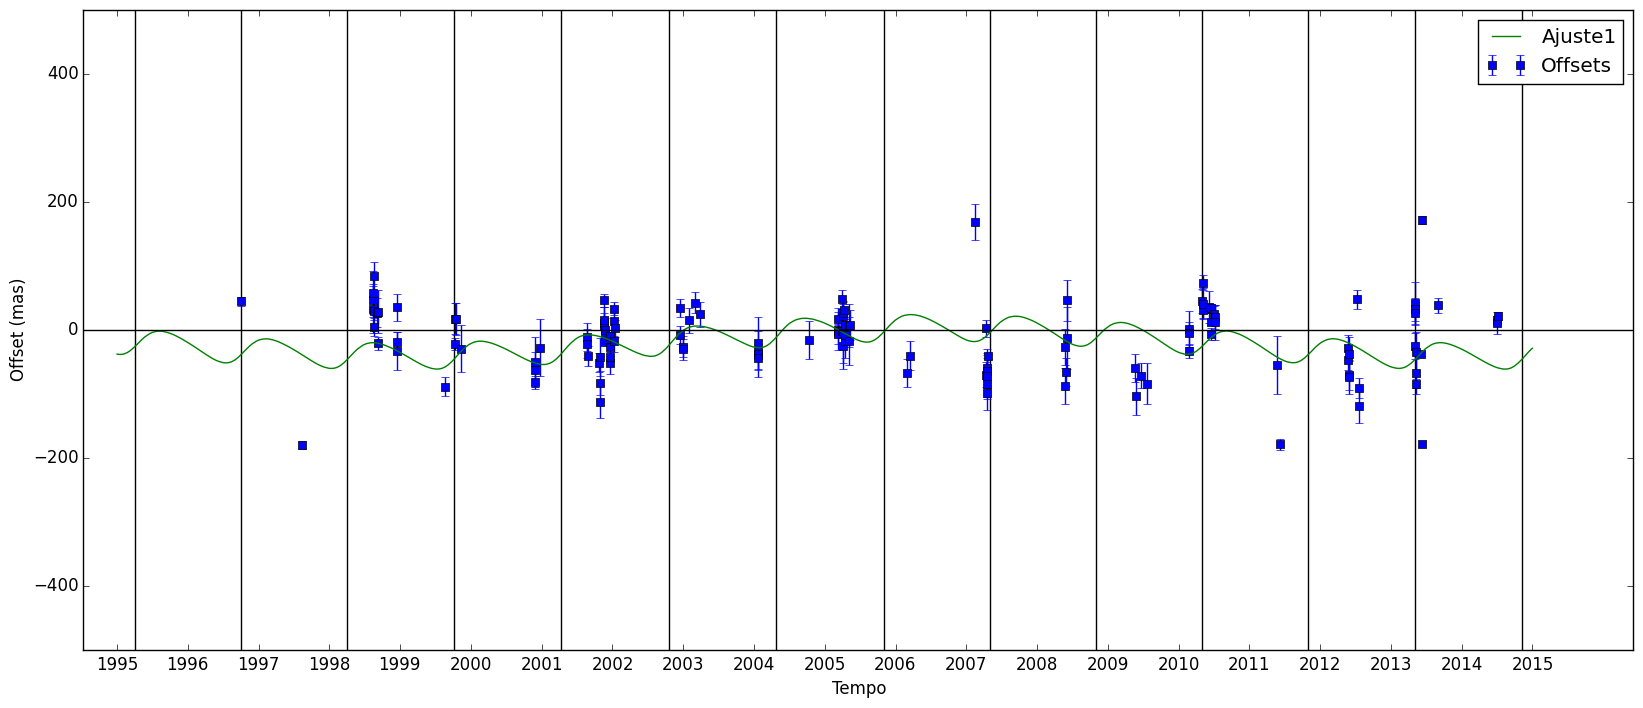
\includegraphics[scale=0.45]{Phoebe/DEC.png} 
\end{figure}

\begin{figure}[h]
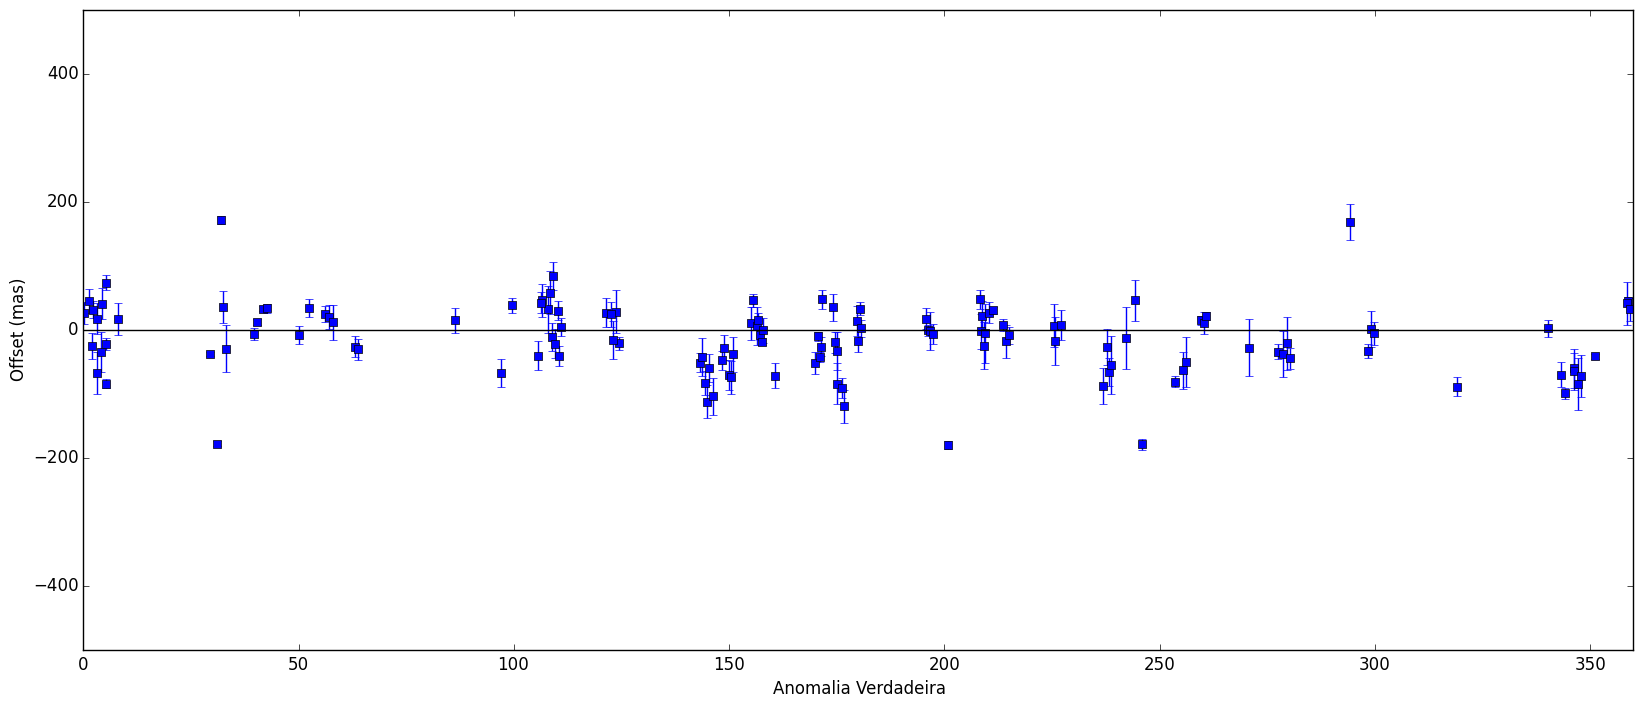
\includegraphics[scale=0.45]{Phoebe/DEC_anom.png}  
\end{figure}

\begin{table}[h!]
\caption{\label{Tab: Phoebe-DEC} Resultados dos ajustes para Phoebe - DEC}
\begin{centering}
\begin{tabular}{cccc}
\hline
\hline
Parâmetro & Com peso & Sem peso & Unidade\tabularnewline
\hline
p[0] & 22 $\pm$ 14 & 20 $\pm$ 8 & mas\\
p[1] & 0.98 $\pm$ 0.01 & 0.95 $\pm$ 0.01 & anos\\
p[2] & 26 $\pm$ 43 & -37 $\pm$ 27 & graus\\
p[3] & 17 $\pm$ 12 & 16 $\pm$ 7 & mas\\
p[4] & 2 $\pm$ 10 & 10 $\pm$ 6 & mas\\
p[5] & -16 $\pm$ 8 & -9 $\pm$ 5 & mas\\
Residuo & 70 & 51 & mas\\
\hline 
\end{tabular} 
\par\end{centering}
\end{table}

\chapter*{Nereida}

\indent \indent Número total de noites: 79.

Não mostro nenhum ajuste pois não encontrei nenhuma função com ajuste razoável. Isso provavelmente se deve pelo fato de não haver observações na metade próxima ao periastro.

\section*{Ascensão Reta}

\begin{figure}[h]
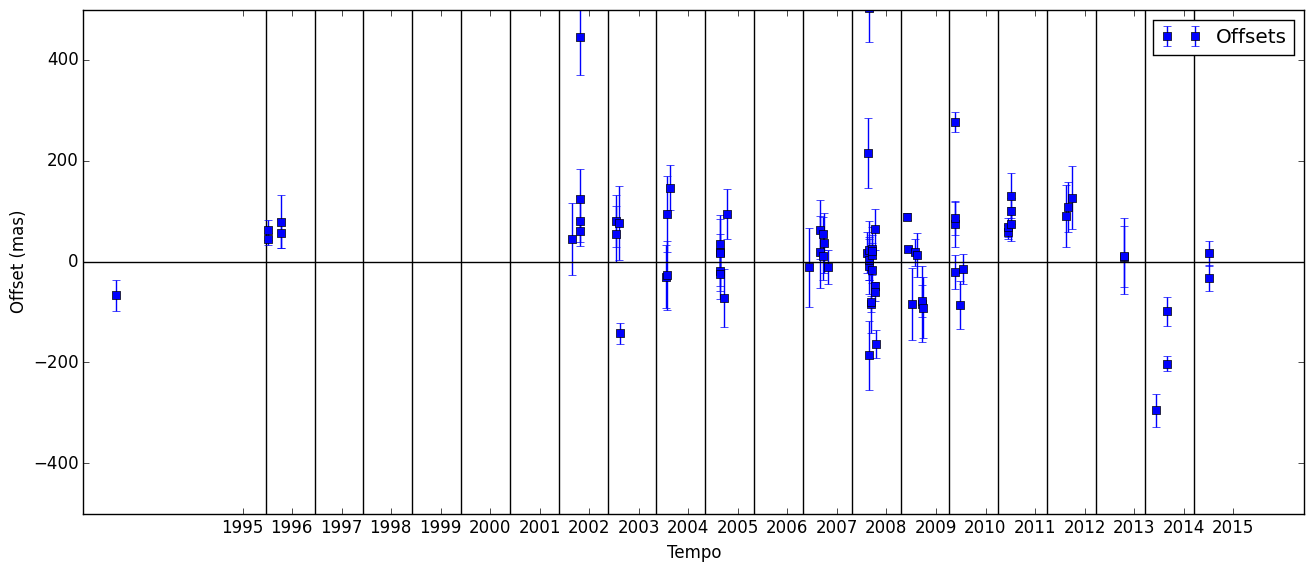
\includegraphics[scale=0.45]{Nereida/RA.png} 
\end{figure}

\begin{figure}[h]
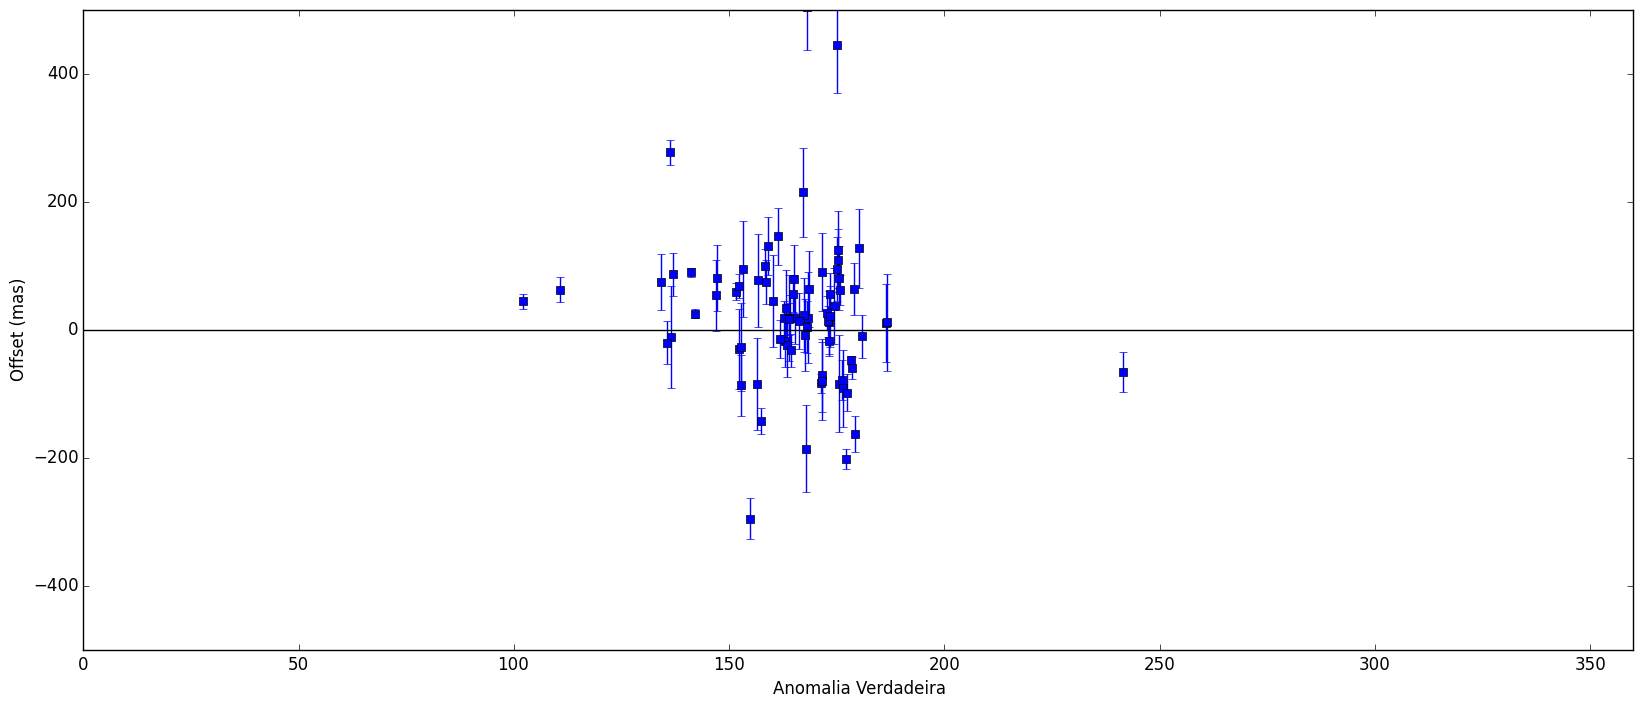
\includegraphics[scale=0.45]{Nereida/RA_anom.png}  
\end{figure}

%\begin{table}[h!]
%\caption{\label{Tab: Nereida-RA} Resultados dos ajustes para Nereida - RA}
%\begin{centering}
%\begin{tabular}{cccc}
%\hline
%\hline
%Parâmetro & Com peso & Sem peso & Unidade\tabularnewline
%\hline
%p[0] & -130 $\pm$ 29 & -46 $\pm$ 25 & mas\\
%p[1] & 11.3 $\pm$ 0.7 & 8 $\pm$ 1 & anos\\
%p[2] & -0.8 $\pm$ 0.3 & -2.8 $\pm$ 0.9 & graus\\
%p[3] & 39 $\pm$ 81 & 39 $\pm$ 81 & mas\\
%p[4] & 193 $\pm$ 119 & -27 $\pm$ 130 & mas\\
%p[5] & 123 $\pm$ 125 & -21 $\pm$ 130 & mas\\
%Residuo & 1427 & 1154 & mas\\
%\hline 
%\end{tabular} 
%\par\end{centering}
%\end{table}

\section*{Declinação}

\begin{figure}[h]
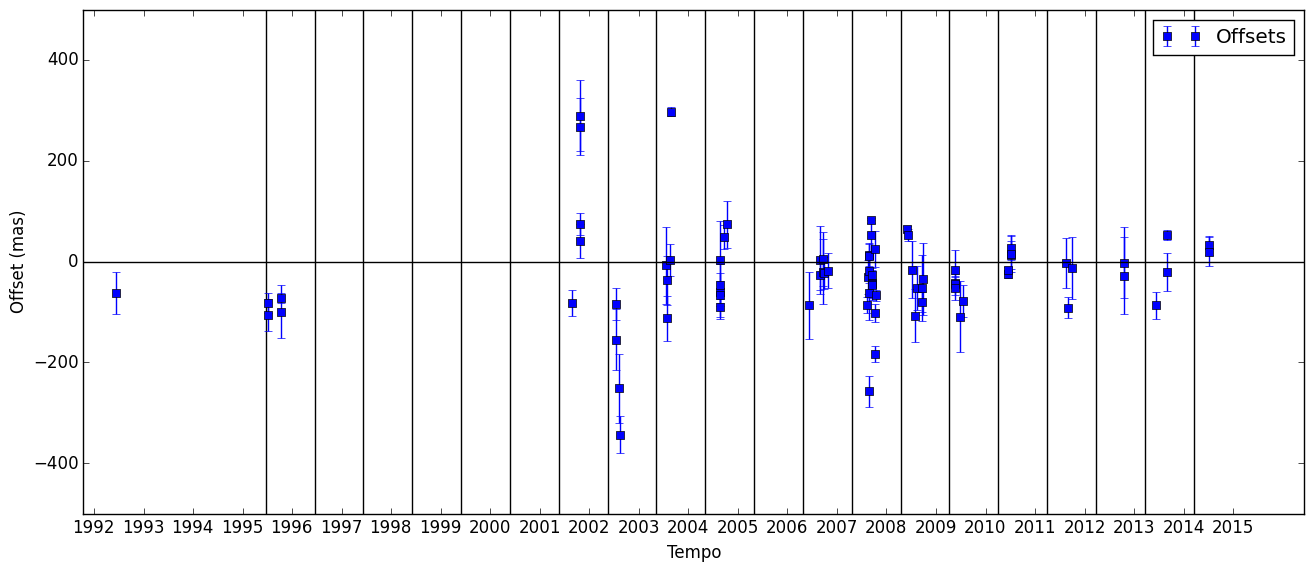
\includegraphics[scale=0.45]{Nereida/DEC.png} 
\end{figure}

\begin{figure}[h]
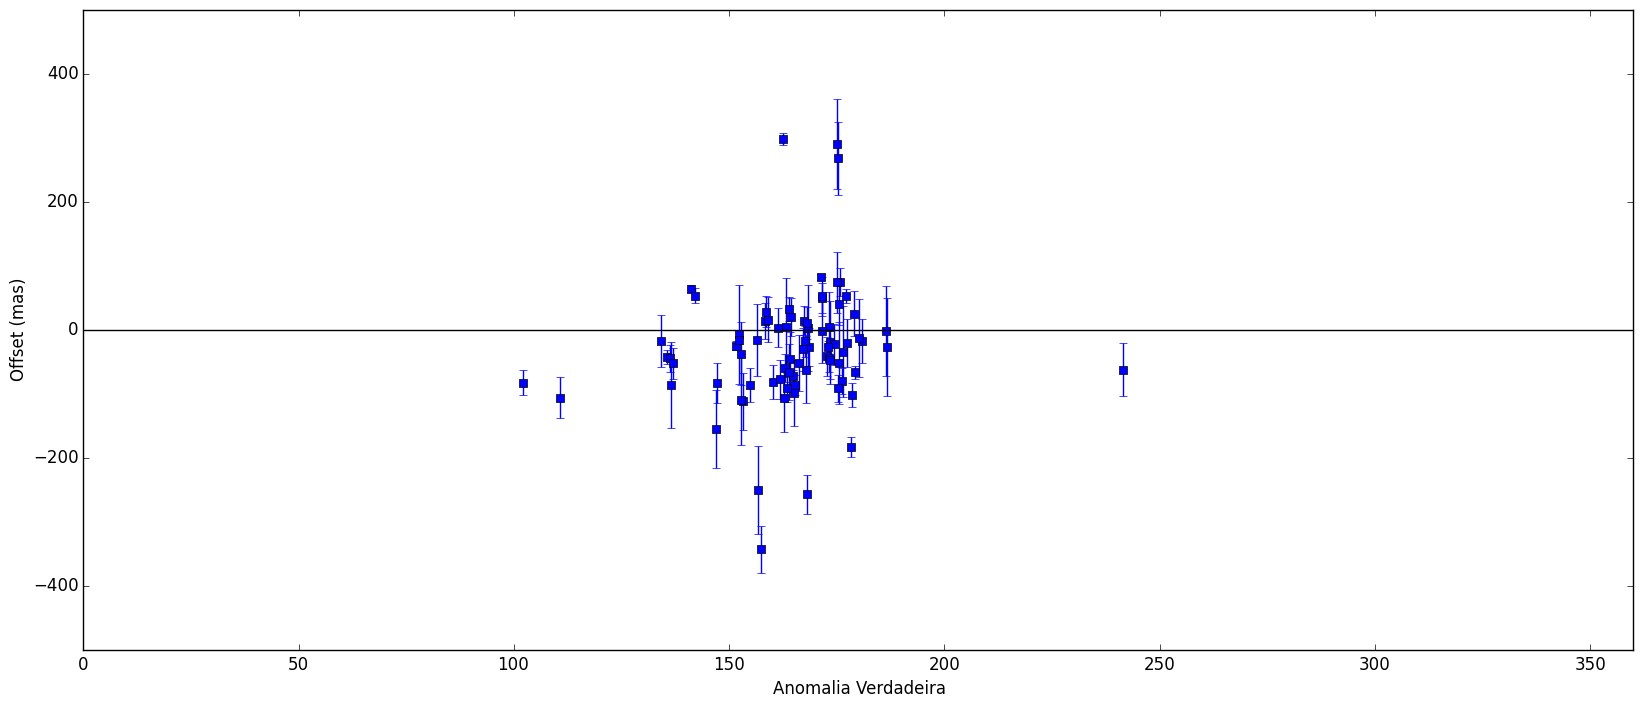
\includegraphics[scale=0.45]{Nereida/DEC_anom.png}  
\end{figure}

%\begin{table}[h!]
%\caption{\label{Tab: Nereida-Dec} Resultados dos ajustes para Nereida - DEC}
%\begin{centering}
%\begin{tabular}{cccc}
%\hline
%\hline
%Parâmetro & Com peso & Sem peso & Unidade\tabularnewline
%\hline
%p[0] & 83 $\pm$ 19 & 21 $\pm$ 17 & mas\\
%p[1] & 14 $\pm$ 2 & -14 $\pm$ 7 & anos\\
%p[2] & -0.1 $\pm$ 0.6 & 1.9 $\pm$ 1.7 & graus\\
%p[3] & 165 $\pm$ 87 & -40 $\pm$ 51 & mas\\
%p[4] & -186 $\pm$ 158 & -63 $\pm$ 92 & mas\\
%p[5] & -182 $\pm$ 172 & -70 $\pm$ 93 & mas\\
%Residuo & 1120 & 820 & mas\\
%\hline 
%\end{tabular} 
%\par\end{centering}
%\end{table}

\end{document}